\documentclass[a4paper]{article}

\setlength{\parindent}{0pt}
\setlength{\parskip}{1em}

\pagestyle{headings}

\usepackage{amssymb}
\usepackage{amsmath}
\usepackage{amsthm}
\usepackage{mathtools}
\usepackage{graphicx}
\usepackage{hyperref}
\usepackage{color}
\usepackage{microtype}
\usepackage{tikz}
\usepackage{pgfplots}
\usepackage{pgfplotstable}

\newcommand{\N}{\mathbb{N}}
\newcommand{\Q}{\mathbb{Q}}
\newcommand{\Z}{\mathbb{Z}}
\newcommand{\R}{\mathbb{R}}
\newcommand{\C}{\mathbb{C}}
\newcommand{\D}{\mathcal{D}}
\renewcommand{\S}{\mathcal{S}}
\renewcommand{\P}{\mathbb{P}}
\newcommand{\F}{\mathbb{F}}
\newcommand{\E}{\mathbb{E}}
\newcommand{\bra}{\langle}
\newcommand{\ket}{\rangle}


\graphicspath{{Image/}}

\hypersetup{
    colorlinks=true,
    linktoc=all,
    linkcolor=blue
}

\theoremstyle{definition}
\newtheorem*{axiom}{Axiom}
\newtheorem*{claim}{Claim}
\newtheorem*{conv}{Convention}
\newtheorem*{coro}{Corollary}
\newtheorem*{defi}{Definition}
\newtheorem*{eg}{Example}
\newtheorem*{lemma}{Lemma}
\newtheorem*{notation}{Notation}
\newtheorem*{prob}{Problem}
\newtheorem*{post}{Postulate}
\newtheorem*{prop}{Proposition}
\newtheorem*{rem}{Remark}
\newtheorem*{thm}{Theorem}

\DeclareMathOperator{\vdiv}{div}
\DeclareMathOperator{\grad}{grad}
\DeclareMathOperator{\curl}{curl}
\DeclareMathOperator{\Ann}{Ann}
\DeclareMathOperator{\Fit}{Fit}
\DeclareMathOperator{\Diag}{Diag}
\DeclareMathOperator{\tr}{tr}
\DeclareMathOperator{\im}{im}
\DeclareMathOperator{\Mat}{Mat}
\DeclareMathOperator{\Log}{Log}
\DeclareMathOperator{\Isom}{Isom}
\DeclareMathOperator{\Mesh}{Mesh}
\DeclareMathOperator{\Sym}{Sym}
\DeclareMathOperator{\Aut}{Aut}
\DeclareMathOperator{\cosech}{cosech}
\DeclareMathOperator{\Card}{Card}
\DeclareMathOperator{\Gal}{Gal}


\setcounter{section}{-1}

\begin{document}

\title{Mathematical Biology}

\maketitle

\newpage

\tableofcontents

\newpage

\section{Miscellaneous}

Course notes online: Julia Gog(www.damtp.cam.ac.uk/research/dd/teaeching, 2013-2017), Peter Haynes(www.damtp.cam.ac.uk/user/phh/mathbio.html)

Moodle page: Handwritten notes by lecture; Matlab/Python programming examples; solved exercises.

This course involves 3 models: Deterministic temporal models (11 lectures), Stochastic temporal models (5 lectures), Deterministic spatio-temporal models (8 lectures).

The focus of this course is biochemical reactions and population processes.

(some introductory speech)

\begin{eg} (1, Transient population)
If we use $n(t)$ to denote the size of a population, we may want to model $\frac{dn}{dt} = f(n)$ by an ODE, or maybe if we have several components $\mathbf{n}(t)$ then we may want to model $\frac{d\mathbf{n}}{dt} = \mathbf{f}(\mathbf{n})$ which is a system of ODEs.

Note that although $n$ should be an integer (discrete), when $n >> 1$ we may model it with continuous equations.
\end{eg}

\begin{eg} (2)
$n \to \partial_t P(n,t) = W \cdot P(n,t)$, Markov processes. Here $P(n,t)$ is a probablity(?), $n$ being a state, and $W$ being the transition matrix.
\end{eg}

\begin{eg} (3)\\
If we include spatial aspect, we may have $n(t)$ becoming $n(x,t)$. Now there might be 'diffusion': $\partial_t n(x,t) = f(n(x,t)) + D \nabla^2 (x,t)$ where $\nabla^2 = \frac{\partial^2}{\partial x^2}$; this is the reaction-diffusion equation.
\end{eg}

\newpage

\section{Birth-death models}
The general idea is that we have a population of size $n(t)$; per capita per unit time, we have births of rate $b$ and deaths of rate $d$. Then we can write $$n(t+\Delta t) = n(t) + bn\Delta t - dn \Delta t$$ So we have an ODE $$\frac{dn}{dt} = (b-d)n = rn$$ where $r = b-d$. This has an easy solution $n(t) = n_0 e^{rt}$, assuming $r$ is a constant. We see that if $r$ is positive then the population grows exponentially, and if $r$ is negative then the population decreases to 0 asymptotically.

Now probably $b$ and $d$ are related to $n$ by $b(n) = bn$ and $d(n) = dn^2$ due to competition. Then we have $$\frac{dn}{dt} = bn-dn^2$$ which we can definitely rewrite as $$\frac{dn}{dt}=\alpha n(1-n)$$ by some change of variable on $n$. Now

\begin{equation*}
\begin{aligned}
\frac{dn}{n(1-n)}&=\alpha dt\\
\implies \frac{dn}{n} + \frac{dn}{1-n} &= \alpha dt\\
\implies \ln n - \ln(1-n) &= \alpha t + c\\
\implies n &= \frac{n_0 e^{\alpha t}}{(1-n_0) + n_0 e^{\alpha t}}
\end{aligned}
\end{equation*}
where we are given that $t=0$, $n=n_0$. If $t \gg \frac{1}{\alpha}$, when $t \to \infty$ we have $n(t) \to 1$. Now we can investigate if the population size is stable, and if it has any fixed points.



Let's now define $\mathbf{n} = (n_1,...,n_p)$, i.e. $p$ populations, and $\frac{d\mathbf{n}}{dt} = \mathbf{f}(\mathbf{n})$. If $\mathbf{n}=\mathbf{n}^*$ is a fixed point, then $\frac{d\mathbf{n}}{dt} = 0$, i.e. $\mathbf{f}(\mathbf{n}) = 0$. Now if we apply a small perturbation $\mathbf{n} = \delta\mathbf{n}^* + \delta \mathbf{n}$, i.e.

\begin{equation*}
\begin{aligned}
\frac{d}{dt} \delta \mathbf{n} &= \mathbf{f} (\mathbf{n}^* + \delta \mathbf{n})\\
a&= \mathbf{f} (\mathbf{n}^*) + \frac{\partial f_i}{\partial n_j} \delta_{nj} + \frac{1}{2} \frac{\partial^2 f_i} {\partial n_j \partial n_k} \delta_{n_j} \delta_{n_k}
\end{aligned}
\end{equation*}
So $\frac{d}{dt} \delta \mathbf{n} = J \cdot \partial \mathbf{n}$, so $\delta n(t) = e^{J t} \cdot \delta n(0)$. If $\lambda_i$'s are the eigenvalues of $J$, we consider the real part of $\lambda_i$: if $Re(\lambda_i)<0$, then  if $p\geq 5$ we only have numerical solutions, if $3 \leq p \leq 5$ we have analytic solutions, and $p=2$ is an easy case (recall $p$ is the number of populations):

$\bullet$ If $p=2$, $\mathbf{n} = (n_1,n_2)$, then 
\begin{equation*}
\begin{aligned}
\frac{d}{dt} \begin{pmatrix} \delta_{n_1} \\
\delta_{n_2}
\end{pmatrix} = \begin{pmatrix}
\frac{\partial f_1}{\partial n_1} & \frac{\partial f_1}{\partial n_2}\\
\frac{\partial f_2}{\partial n_1} & \frac{\partial f_2}{\partial n_2}
\end{pmatrix} \cdot \begin{pmatrix}
\delta_{n_1}\\
\delta_{n_2}
\end{pmatrix}
\end{aligned}
\end{equation*}
Where the matrix is $J$. Now we have $\lambda_1\lambda_2 =\det J$ and $\lambda_1 + \lambda_2 = \tr J$. Determined by the signs of those two, we have different possible behaviours:

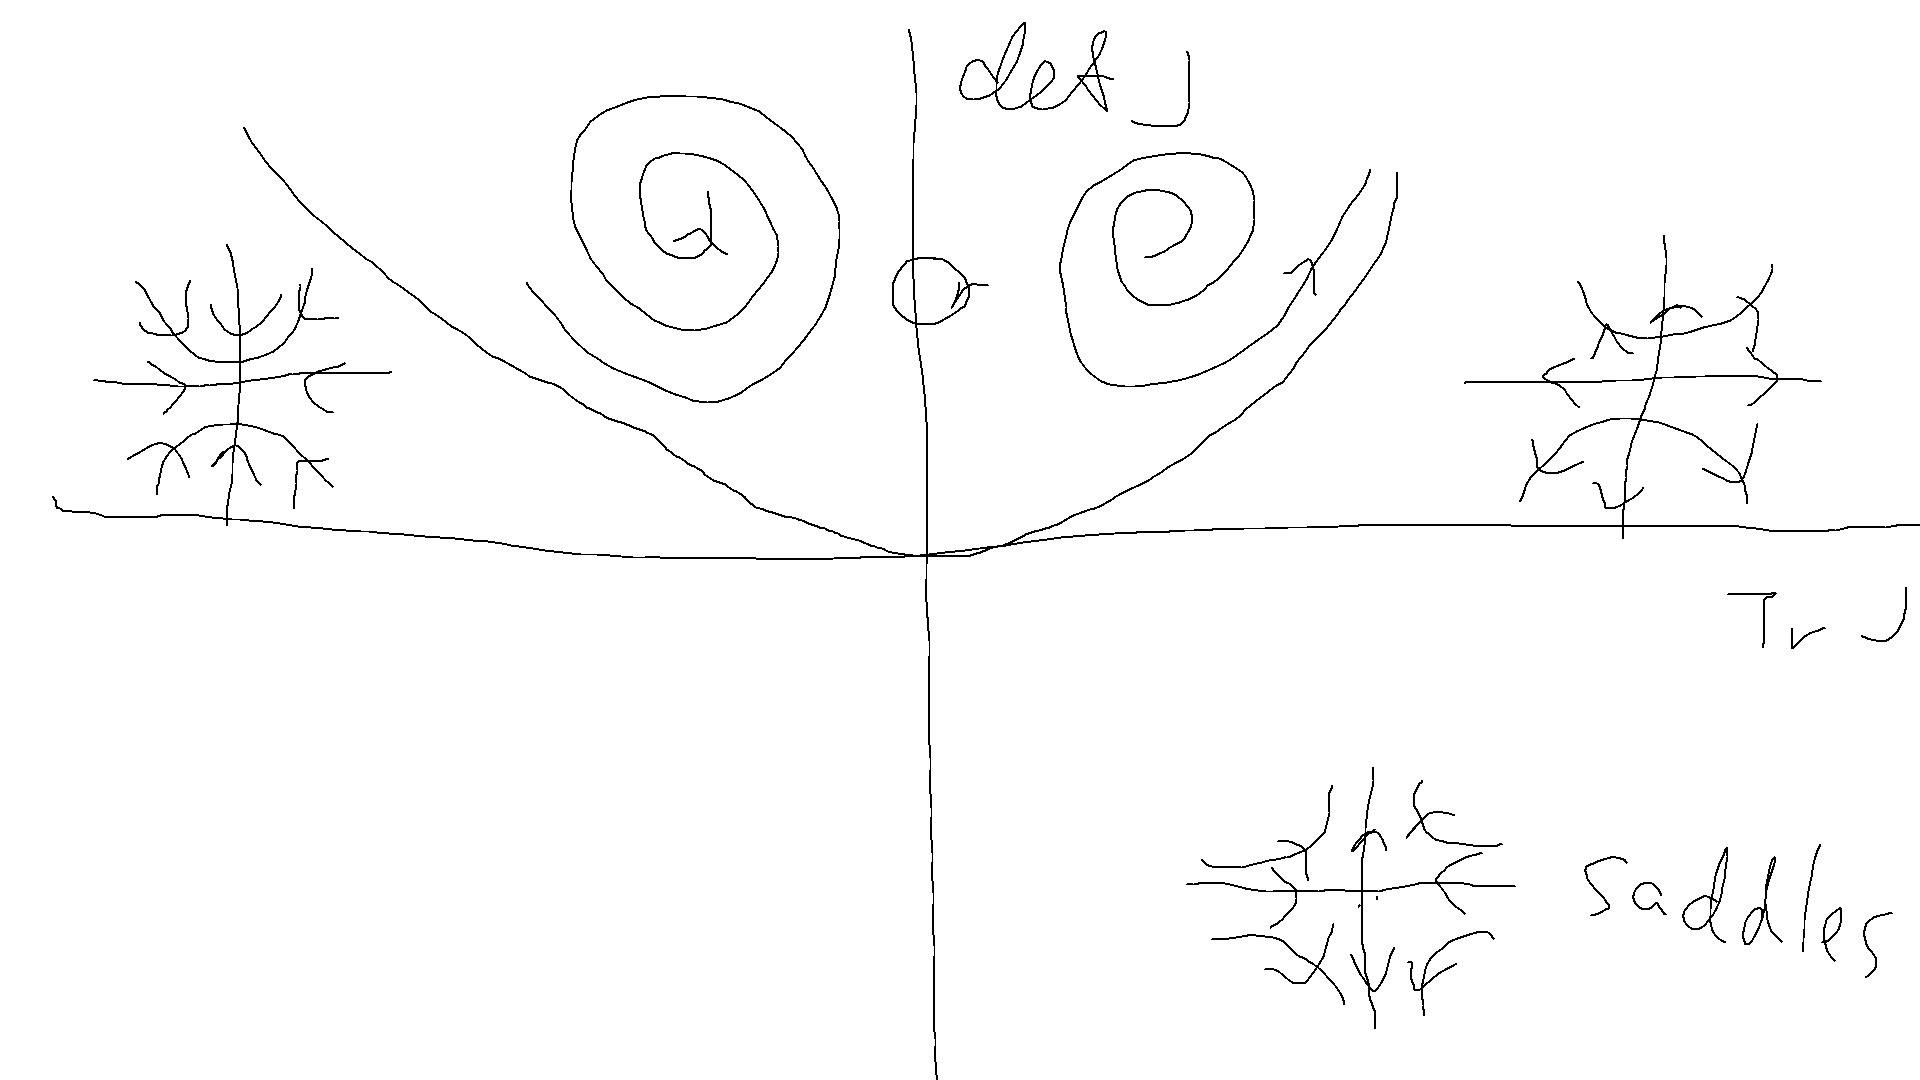
\includegraphics[scale=0.5]{image/Bio_01.png}

Now let's consider the spread of Dengue. There are several processes going on at the same time:

(1) Mosquitos carry dengue;\\
(2) Wolbachia infect mosquitos;\\
(3) Infected mosquitos do not transmit dengue;\\
(4) Wolbachia transmission only across generations.

Question: will an intially infected population of mosquitos eventually spread over the entire population as $t \to \infty$?

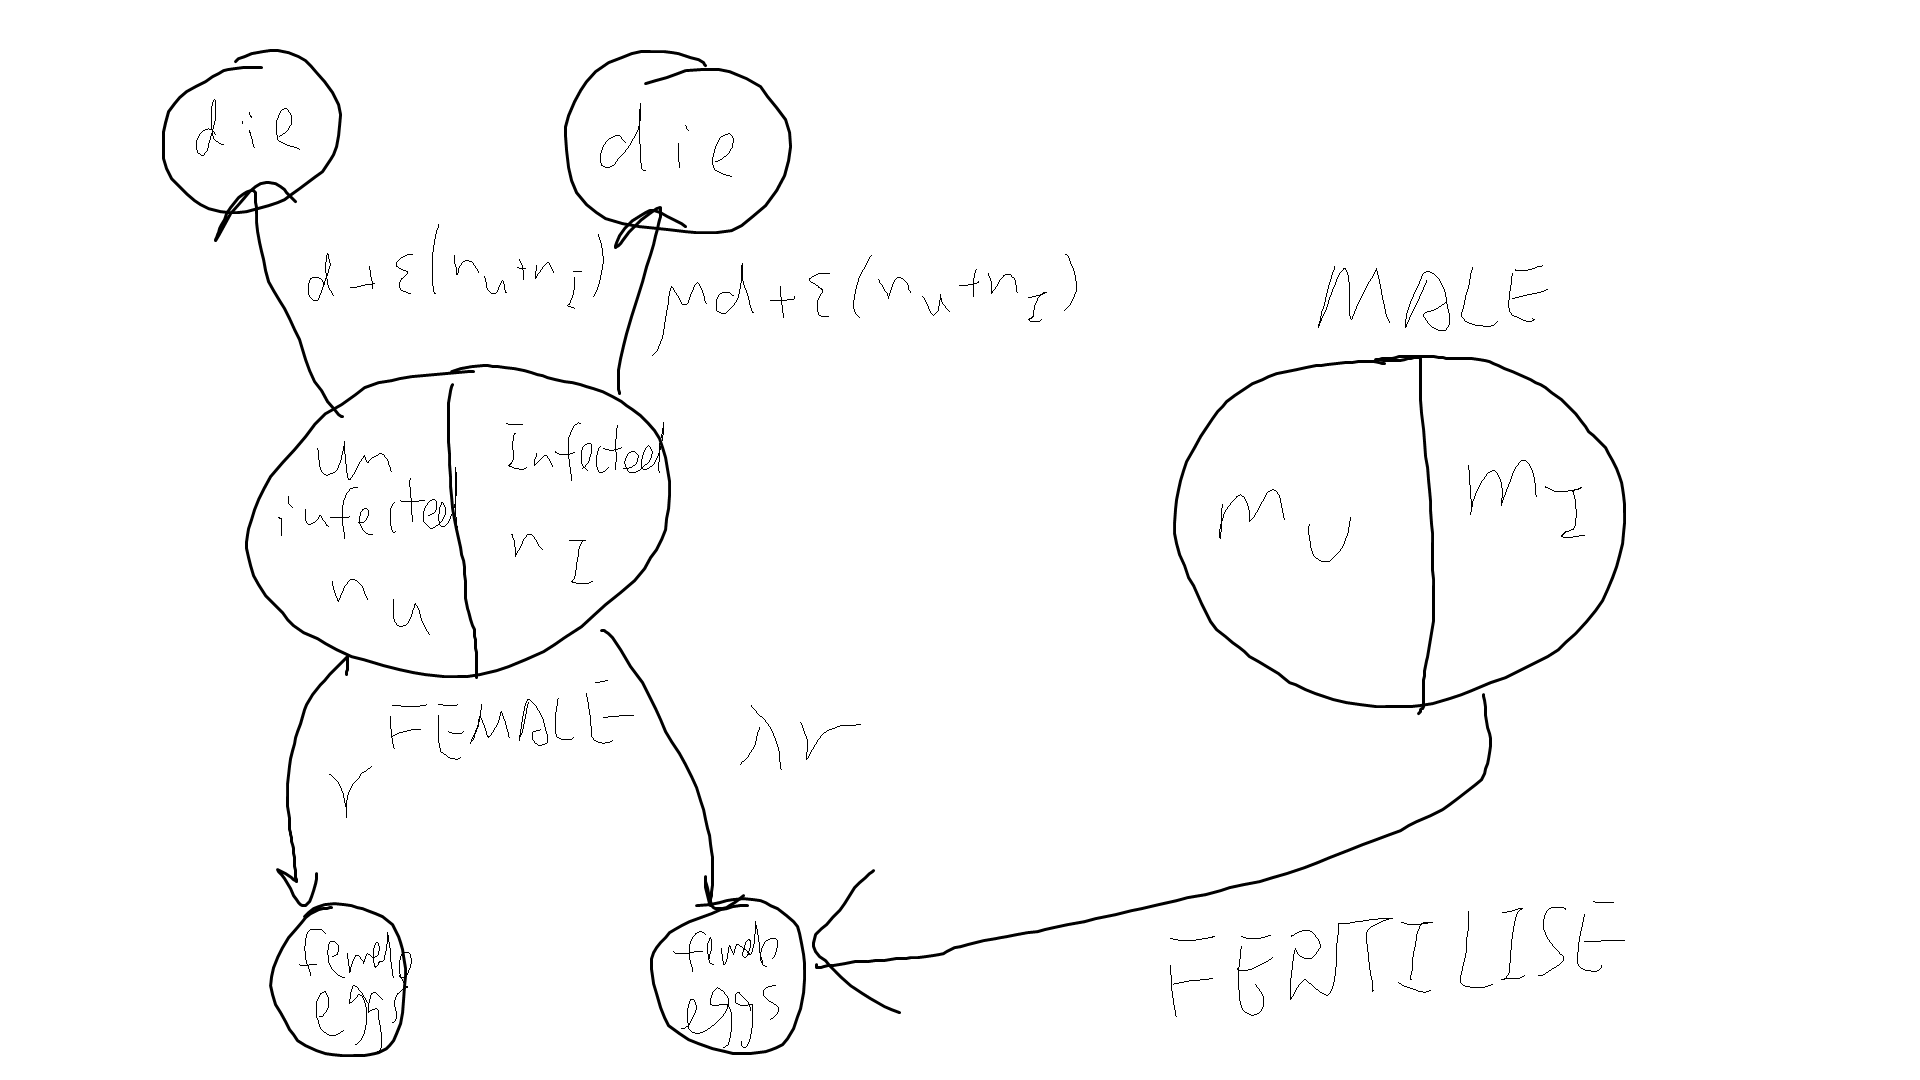
\includegraphics[scale=0.7]{image/Bio_02.png}

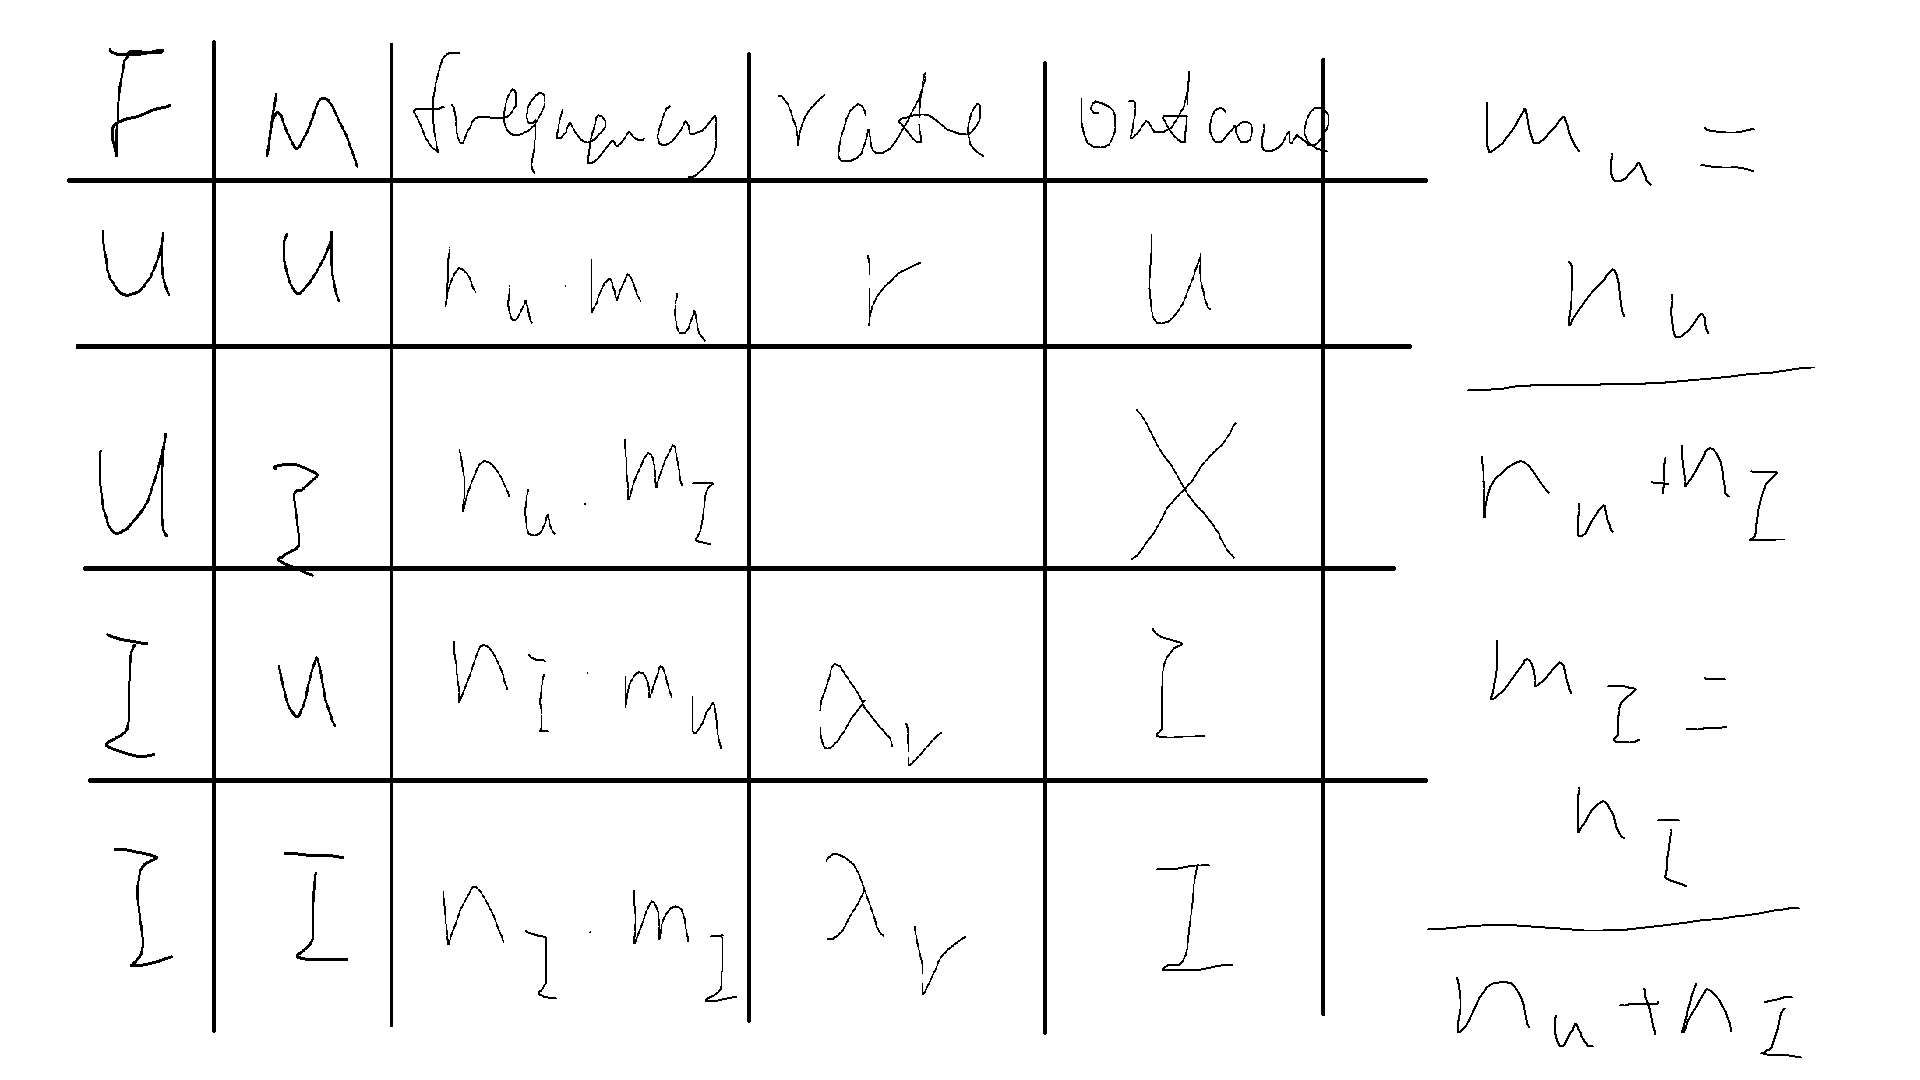
\includegraphics[scale=0.5]{image/Bio_03.png}

We always assume that there are enough males to fertilise the female eggs.

Now consider $\frac{d}{dt}$ of $n_U$ and $n_I$ (uninfected and infected females). From the above tables we should be able to get (hopefully)

\begin{equation*}
\begin{aligned}
\frac{d}{dt} n_U &= r n_U \frac{n_U}{n_U + n_I} - dn_U - \varepsilon (n_U+n_I) n_U\\
\frac{d}{dt} n_I &= \lambda r n_I \frac{n_U}{n_U + n_I} + \lambda r n_I \frac{n_I}{n_U + n_I} - \mu d n_I - \varepsilon (n_U+n_I) n_I \ (*)
\end{aligned}
\end{equation*}
This is our model when $p=2$. The term with $\varepsilon$ is the death rate associated with competition.

We'll try to simplify these equations. By rescaling the time as $t \to rt$, and rescaling the population as $n \to \frac{\varepsilon}{r} n$, we get (?)
\begin{equation*}
\begin{aligned}
\frac{d}{dt} n_U &= n_U \frac{n_U}{n_U + n_I} - \frac{d}{r} n_U - (n_U+n_I) n_U\\
&= n_U\left[\frac{n_U}{n_U+n_I} - \frac{d}{r} - (n_U+n_I)\right] \ (1)
\end{aligned}
\end{equation*}
and the second equation becomes (???)
\begin{equation*}
\begin{aligned}
\frac{d}{dt} n_I = n_I \left[\lambda - \mu \frac{d}{r} - (n_U+n_I)\right] \ (2)
\end{aligned}
\end{equation*}

We'd like to see that the model has at least the fixed points $\mathbf{n}^* = (n^*_U,0)$ and $(0,n^*_I)$. The lecture then somehow defines
\begin{equation*}
\begin{aligned}
n^*_I &= \lambda - \mu \frac{d}{r}\\
n^*_U &= 1-\frac{d}{r}
\end{aligned}
\end{equation*}
so that our differential equations become
\begin{equation*}
\begin{aligned}
\frac{d}{dt} n_U &= n_U \left[n^*_U - \frac{n_I}{n_U+n_I} - (n_U+n_I)\right]\\
\frac{d}{dt} n_I &= n_I \left[n^*_ - (n_U+n_I)\right]
\end{aligned}
\end{equation*}
which has fixed points $(0,0),(n^*_U,0),(0,n^*_I),(n^*_I(1-n^*_I-n^*_U),n^*_I(n^*_U-n^*_I))$. The first is unstable, the second two are stable and the last fixed point is a saddle. This is disappointing because we want a small infection to be spread out to the whole population, but in that case the second fixed point needs to be unstable.

Global analysis:

We can plot the flow of the ode system
\begin{equation*}
\begin{aligned}
\frac{d}{dt} {n_U \choose n_I} = {{f_U(n_U,n_I)} \choose {f_I(n_U,n_I)}}
\end{aligned}
\end{equation*}
This is usually done by programming. We'll try to sketch the flow of this model:

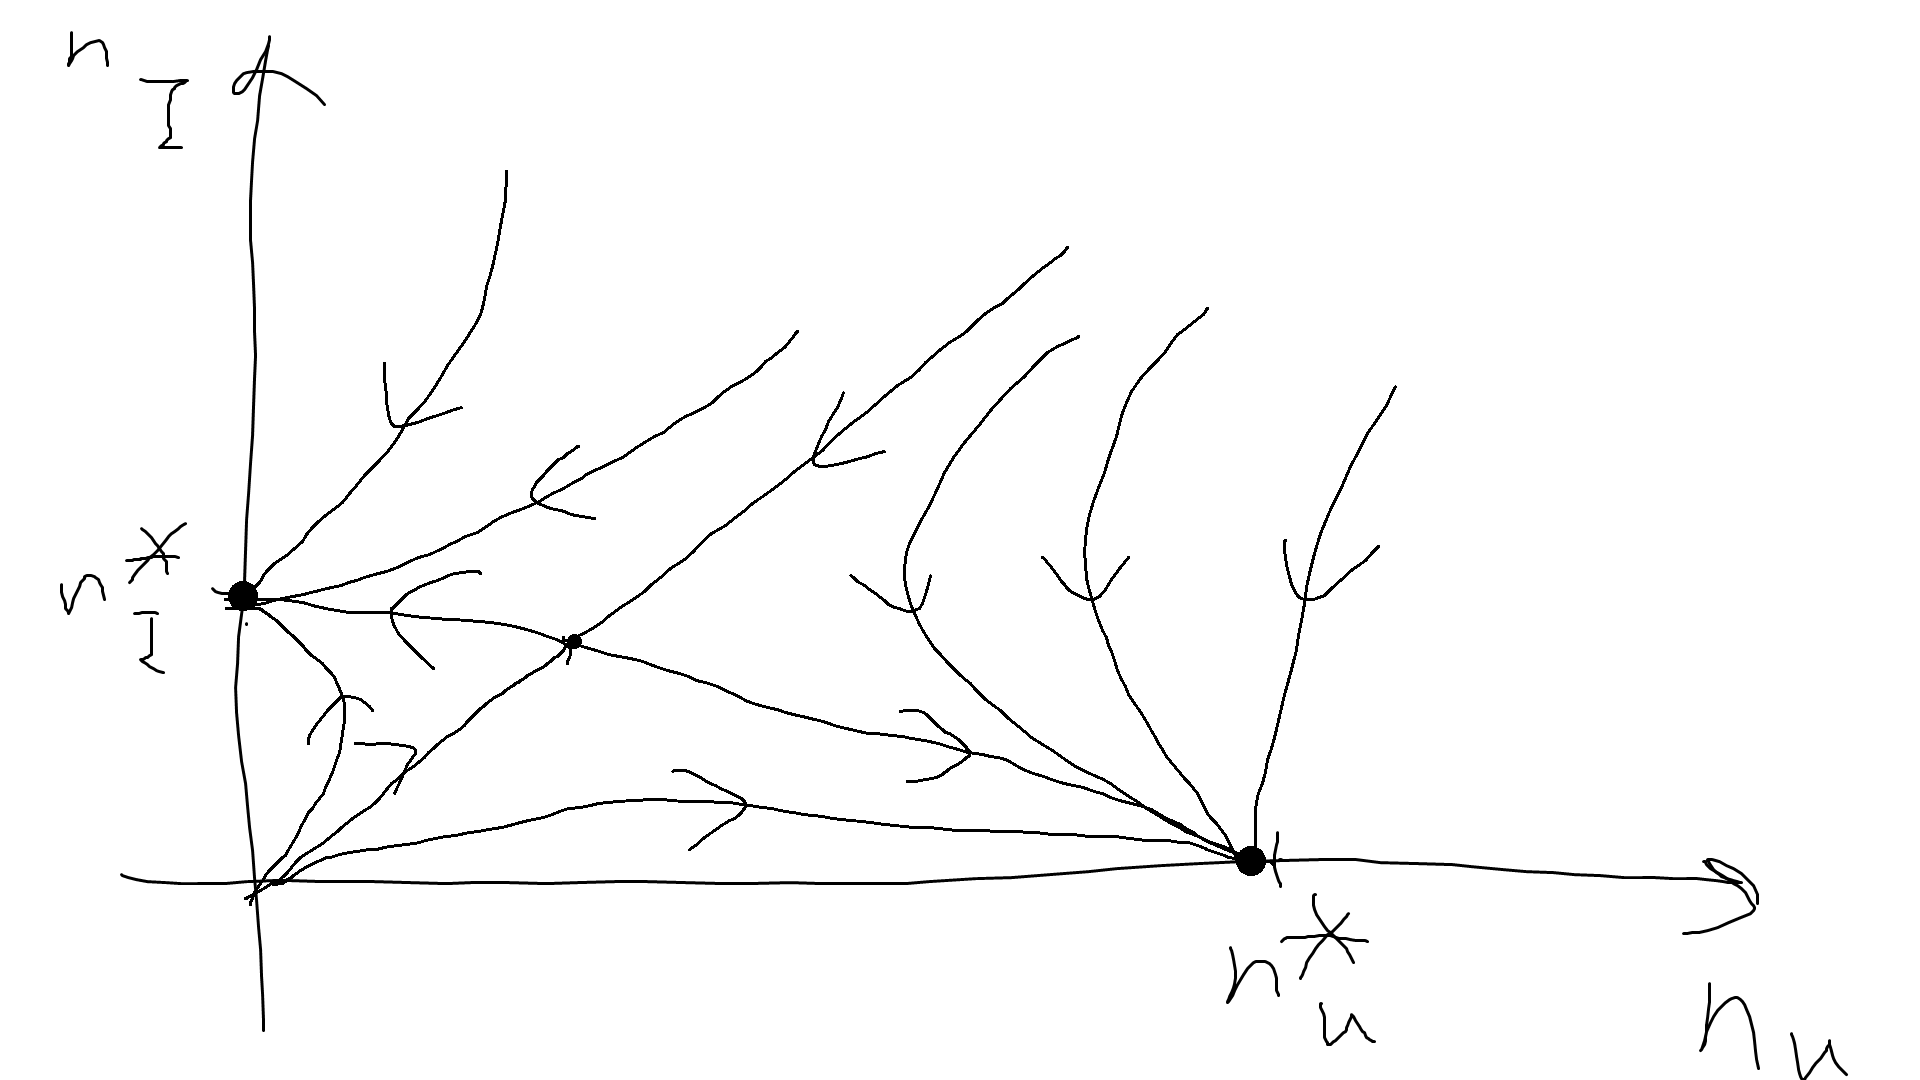
\includegraphics[scale=0.5]{image/Bio_04.png}

Qualitative behaviour: we need a finite (large) $n_I(0)$ (in order to converge to $(n^*_I,0)$).

For quantitative part we can only do numerical integrations.

Now we consider an epidemic model, where each individual may pass through three phases: susceptibles, infectives, recovered (compartment models -- same individual for different phases). We use $S(t),I(t),R(t)$ to denote the population of each of them. 

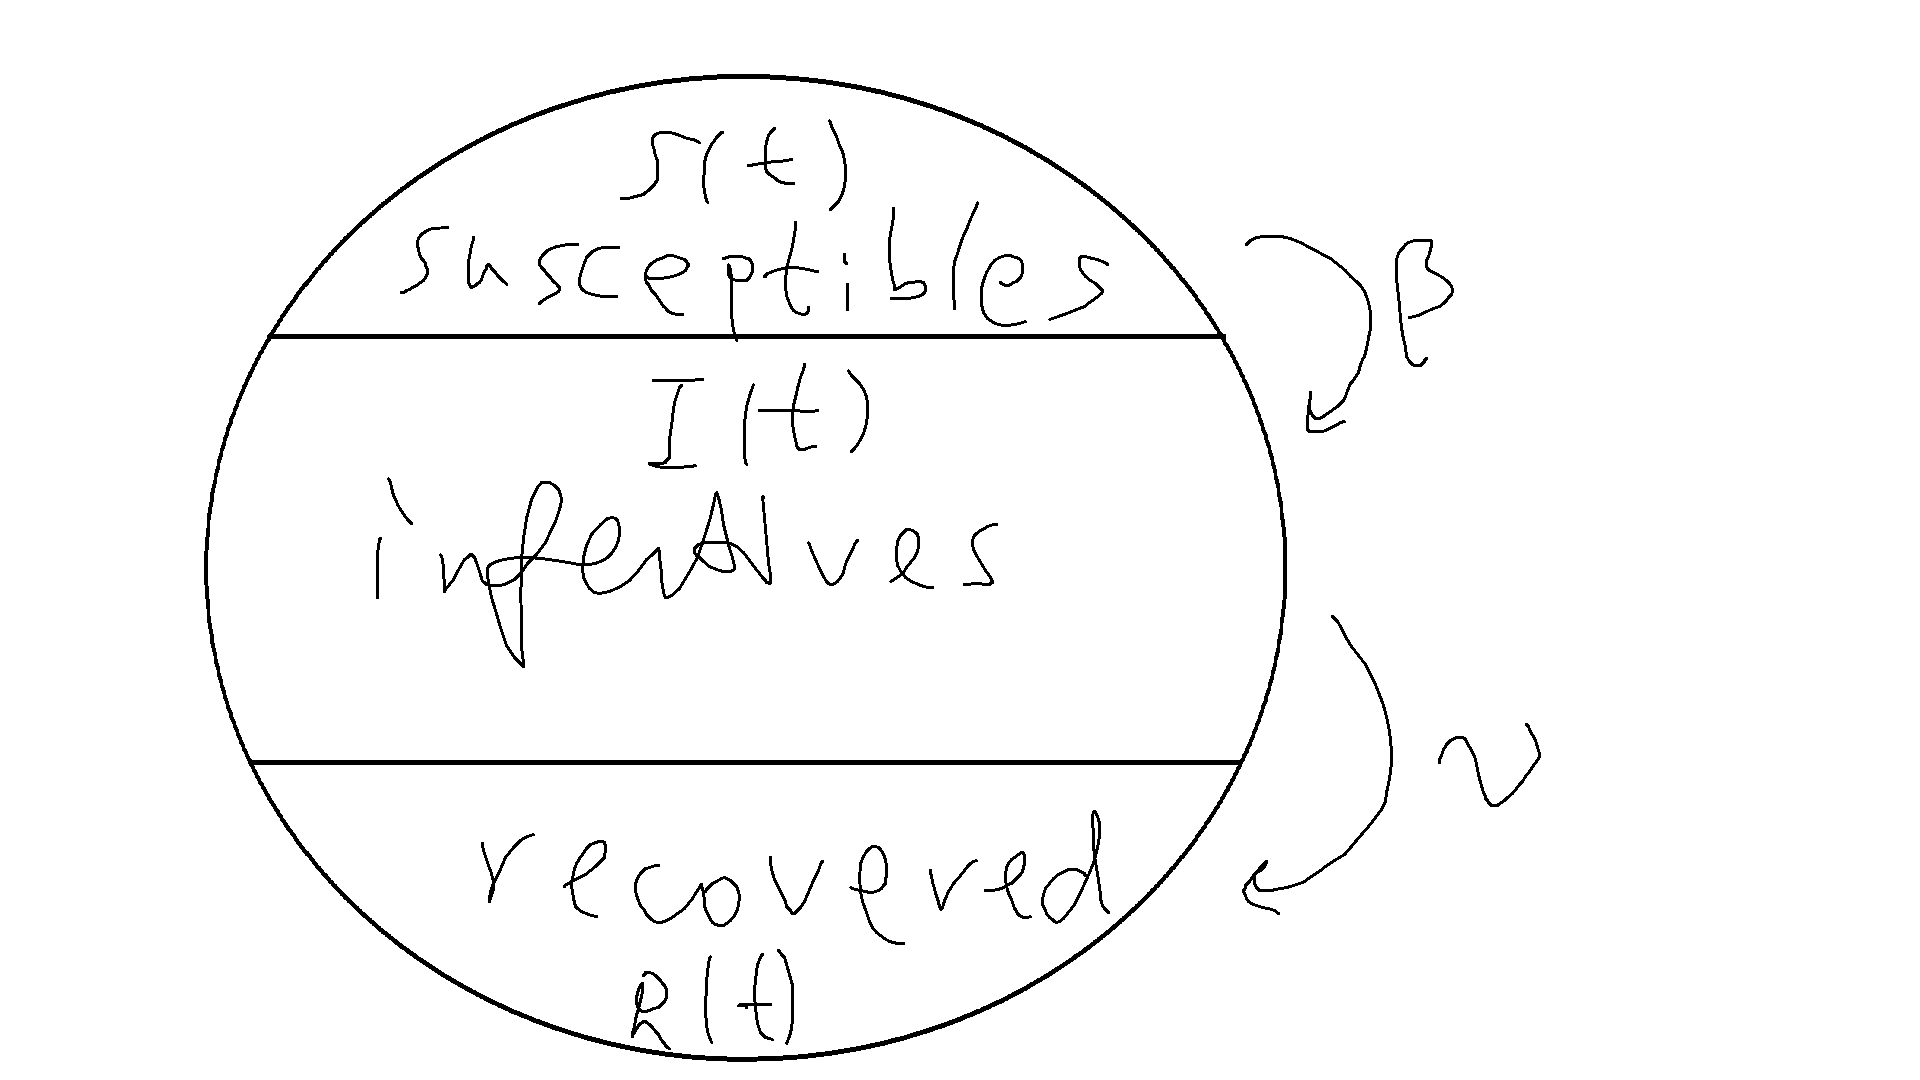
\includegraphics[scale=0.5]{image/Bio_05.png}

Now we want to know what is the rate of their change. We use biological datum, from which we know there is a per capita infection rate $\beta$, a recovery rate $\nu$, so in conclusion we have
\begin{equation*}
\begin{aligned}
\frac{d}{dt} S &= -\beta SI\\
\frac{d}{dt} I &= \beta SI - \nu I\\
\frac{d}{dt} R &= \nu 
\end{aligned}
\end{equation*}
Also we expect the population to be closed, i.e. the total population should not change over time (unlike the previous model), so 
\begin{equation*}
\begin{aligned}
\frac{d}{dt}(S+I+R) = 0
\end{aligned}
\end{equation*}
Which is true. So it's sufficient to look at just two equations,
\begin{equation*}
\begin{aligned}
\frac{dS}{dt} &= -\beta SI\\
\frac{dI}{dt} &= \beta SI - \nu I
\end{aligned}
\end{equation*}
What are the questions we want to ask? We may want to know:\\
$\bullet$ When can you have an \emph{outbreak}, i.e. $\frac{dI}{dt}>0$;\\
$\bullet$ What is the final size of the outbreak?\\
$\bullet$ What vaccination strategy would work best?\\
$\bullet$ Endemic $\implies I^*>0$, finite number of $I$ in steady state.

For obvious reason we call this the "SIR model".

(Q1)\\
at $t=0$, $\frac{d}{dt}I = [\beta S(0) - \nu] \cdot I(0)$, so $\frac{\beta}{\mu}S(0) > 1 \implies \frac{\beta N}{\nu}>1 = \mathcal{R}_0$, the reproduction ratio, or the mean number of susceptibles infected per infective. 

(Q2)\\
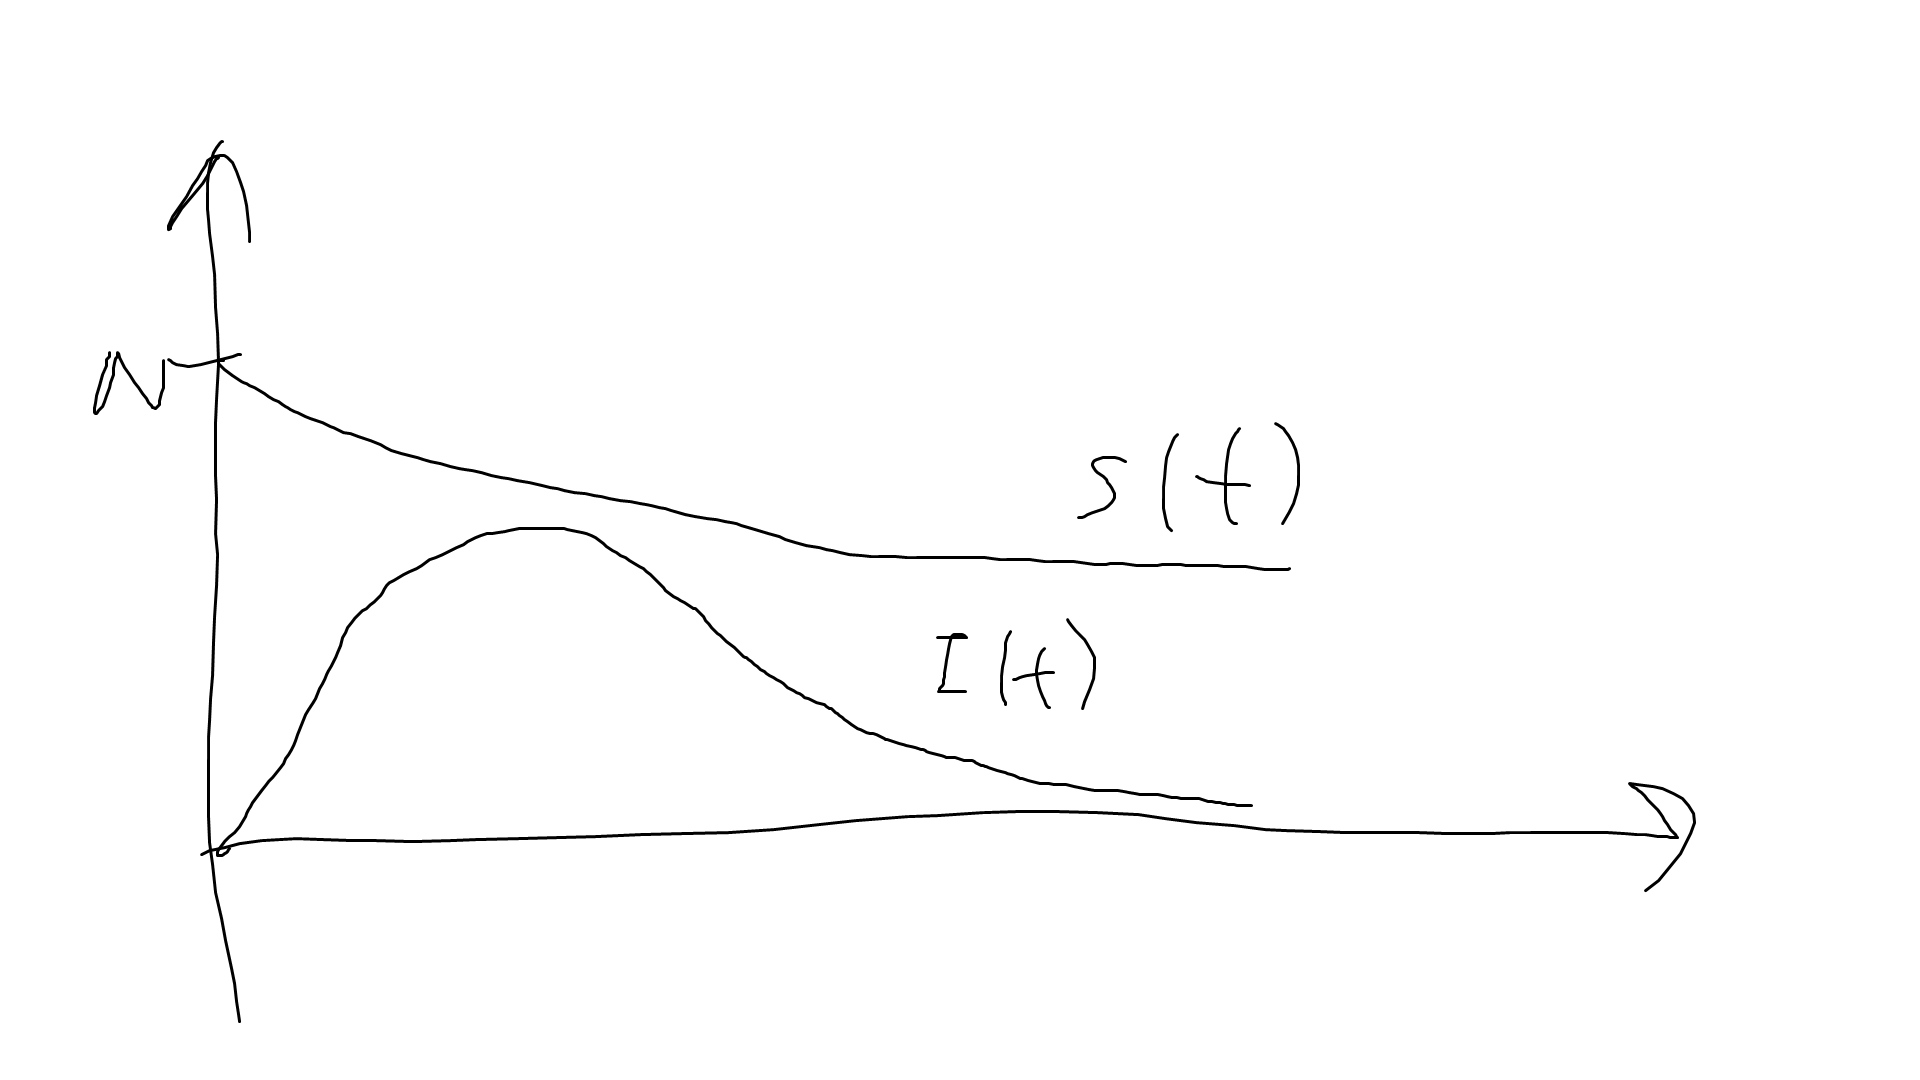
\includegraphics[scale=0.5]{image/Bio_06.png}
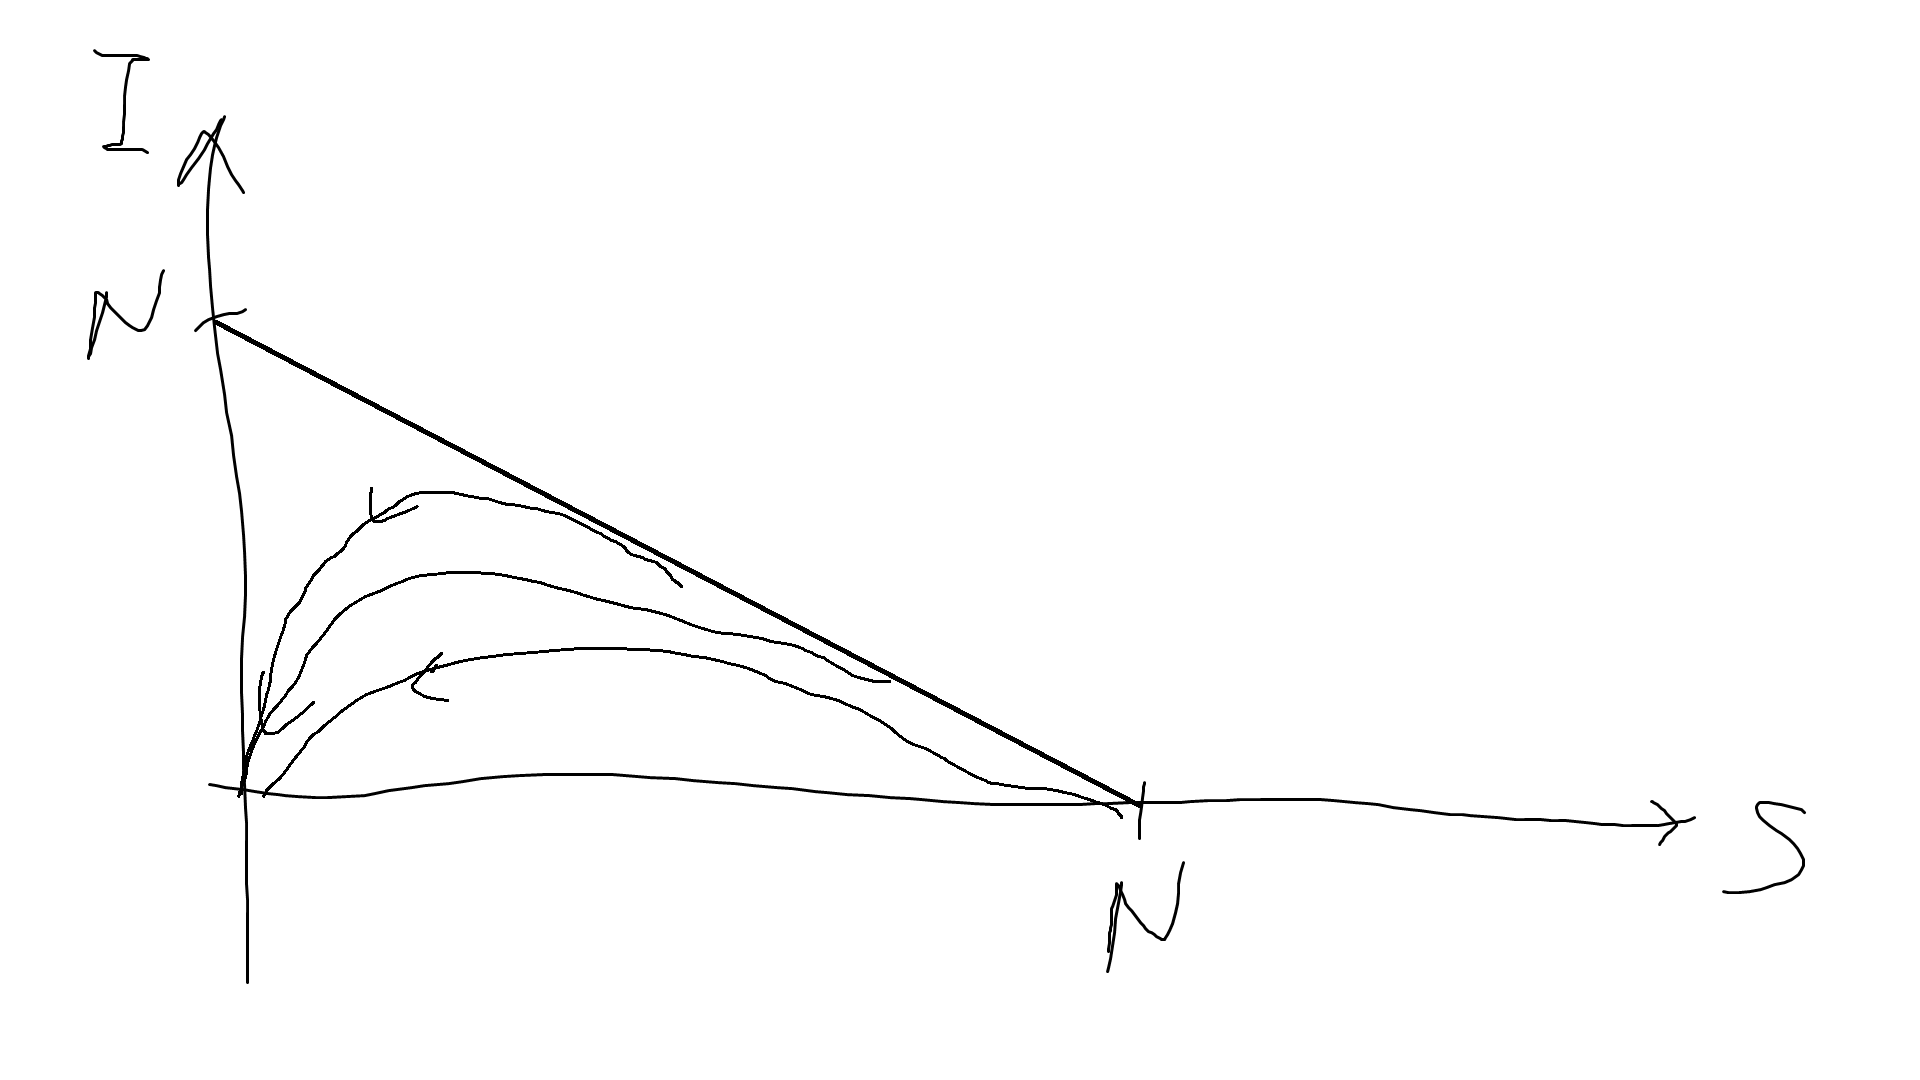
\includegraphics[scale=0.5]{image/Bio_07.png}
We had $dS = -\beta SI dt$, $dI = (\beta SI - \nu I) dt$, so
\begin{equation*}
\begin{aligned}
\frac{dI}{dS} &= \frac{(\beta SI - \nu I)}{-\beta SI} = -1 + \frac{\nu}{\beta} \cdot \frac{1}{S}\\
&= \frac{N}{\mathcal{R}_0} \cdot \frac{1}{S} - 1
\end{aligned}
\end{equation*}
So
\begin{equation*}
\begin{aligned}
I=\frac{N}{\mathcal{R}_0} \ln S - S + \text{ const}
\end{aligned}
\end{equation*}
Now $I(t)-I(0) = \frac{N}{\mathcal{R}_0} \ln \frac{S(t)}{S(0)} - (S(t)-S(0))$. As $t \to \infty$, $S(t) = \sigma N$ ($\sigma < 1$, $I(t) \to 0$. So
\begin{equation*}
\begin{aligned}
0 &= \frac{N}{\mathcal{R}_0} \ln \sigma - (\sigma N-N)\\
\sigma - \frac{1}{\mathcal{R}_0} \ln \sigma &= 1
\end{aligned}
\end{equation*}
We can rewrite the second equation as $\mathcal{R}_0 (\sigma-1) = \ln \sigma$. Clear $\sigma = 1$ is a solution, but we are not interested in that. For $\mathcal{R}_0 \gg 1$, $\sigma \approx e^{-\mathcal{R}_0}$.(by sketching curves below and analyze intersections?)
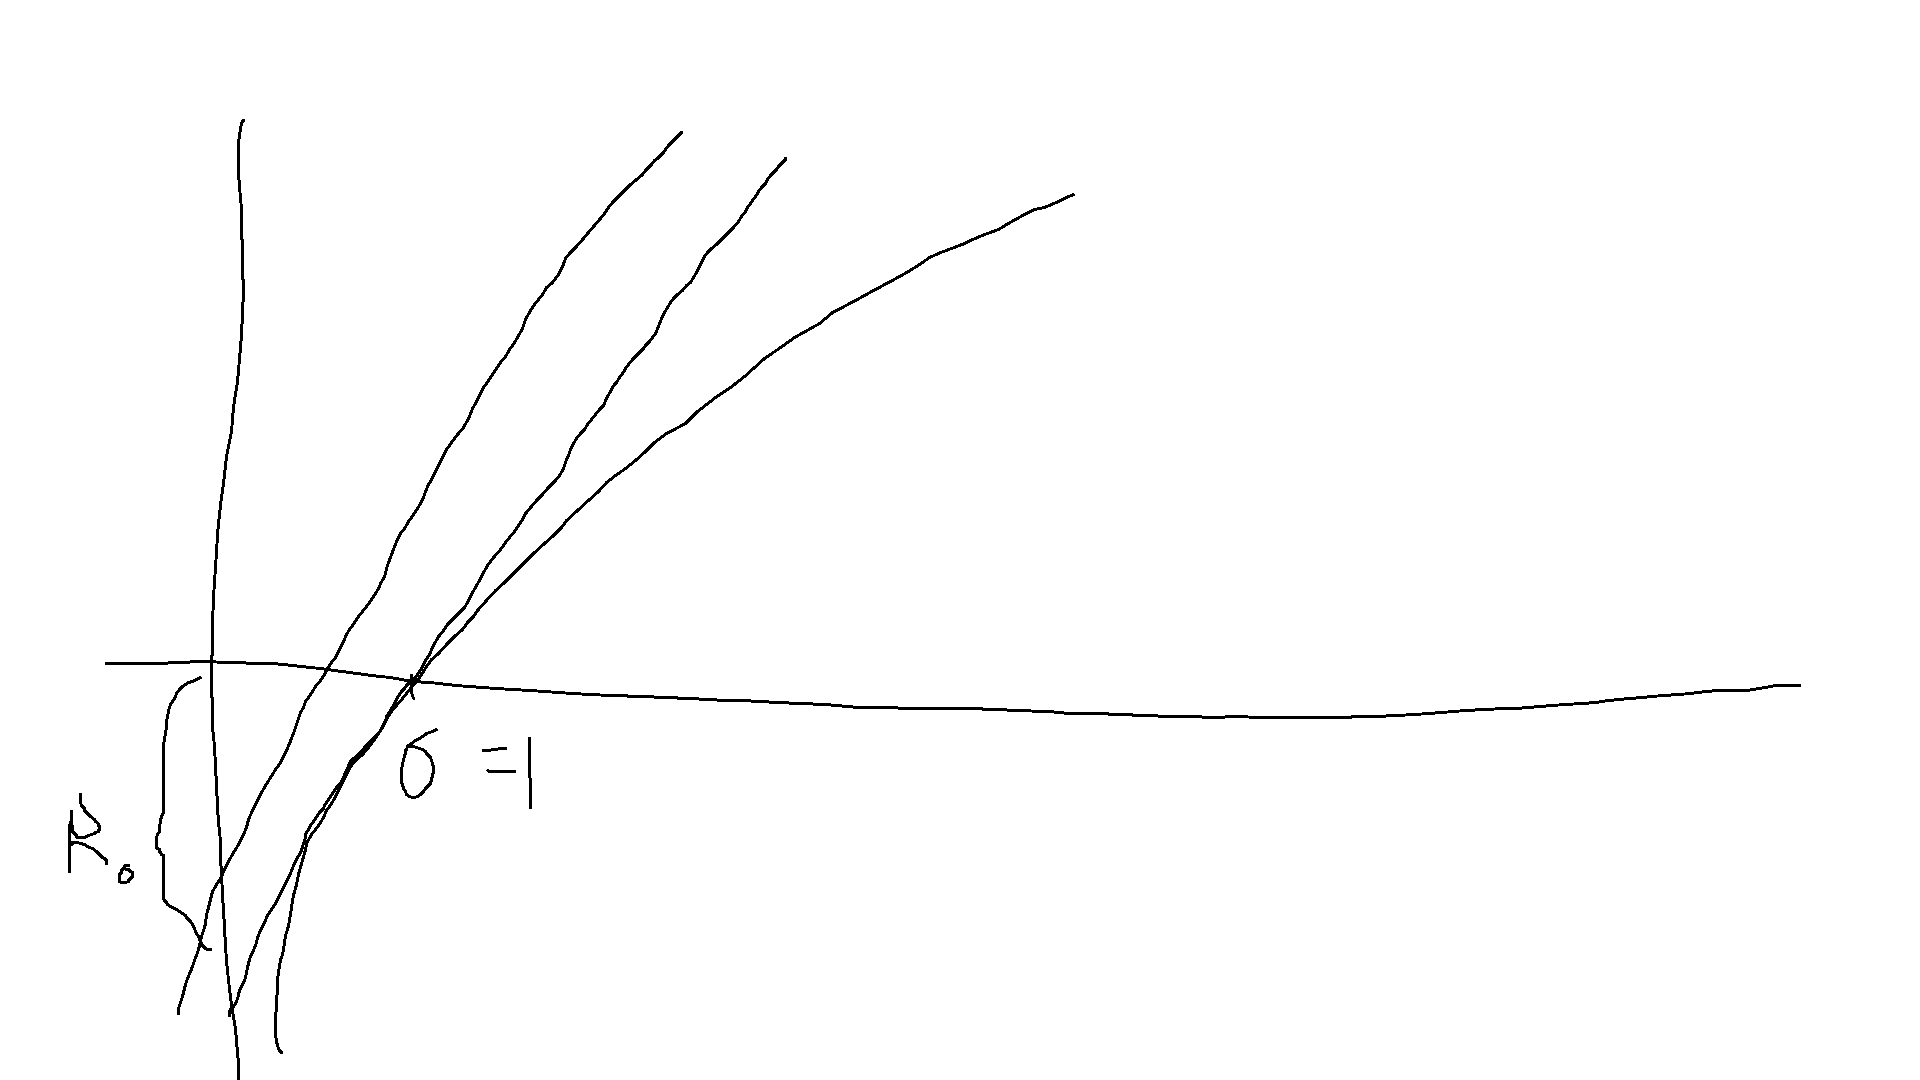
\includegraphics[scale=0.5]{image/Bio_08.png}

Insight: in any epidemic, only a fraction of the population is infected. Size of the epidemic = $(1-\sigma)N$.

(Q3)\\
Vaccination? We can use pre-vaccination, i.e. vaccinate in anticipation of an outbreak. Let $p$ be the fraction of the population being vaccinated. At $t=0$ we have
\begin{equation*}
\begin{aligned}
S(0) \approx (1-p)N\\
\frac{\beta}{\nu} S(0) > 1 \implies \frac{\beta}{\nu} (1-p)N = (1-p)\mathcal{R_0} > 1
\end{aligned}
\end{equation*}
so $p>1-\frac{1}{\mathcal{R}_0}$.
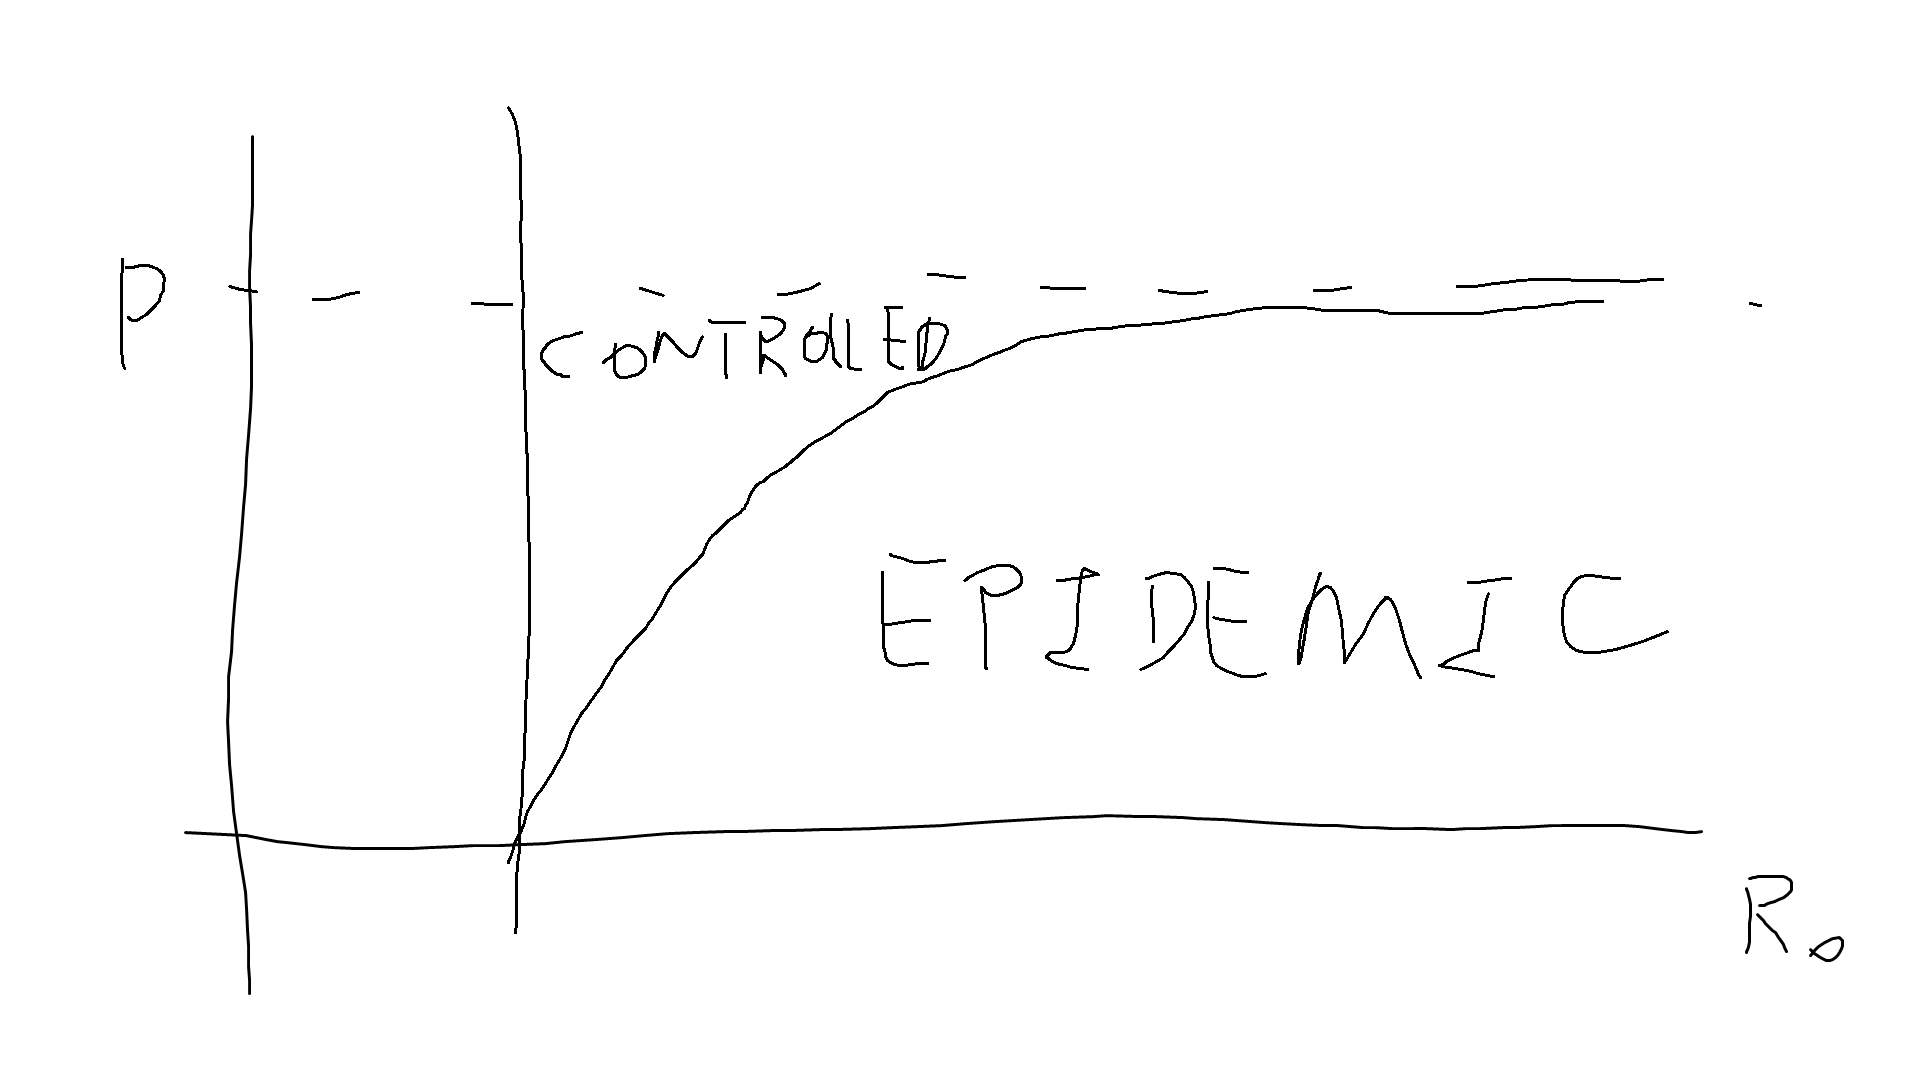
\includegraphics[scale=0.5]{image/Bio_09.png}

(Q4)\\
Endemic: $I(t) \to I^* > 0$ as $t \to \infty$.\\
Biological datum: suppose we have a finite rate of birth of $S$, and of death of $S,I,R$. Now
\begin{equation*}
\begin{aligned}
\frac{d}{dt} S = -\beta SI - \mu S + \mu N\\
\frac{d}{dt} I = \beta SI - \nu I - \mu I\\
\frac{d}{dt} R = \nu I - \mu R
\end{aligned}
\end{equation*}
at $t=0$, $\mathcal{R} = \frac{\beta}{\nu+\mu}N$(??). So
\begin{equation*}
\begin{aligned}
S^* &= \frac{\mu+\nu}{\beta} = \frac{N}{\mathcal{R}_0}\\
I^* &= \frac{\mu(N-S^*)}{\beta S^*} = \frac{\mu}{\beta}(\mathcal{R}_0-1)
\end{aligned}
\end{equation*}
We had a Jacobian (?)
\begin{equation*}
\begin{aligned}
J=\begin{pmatrix}
-\beta I - \mu & -\beta S\\
\beta I & \beta S - \nu - \mu
\end{pmatrix}
\end{aligned}
\end{equation*}
so
\begin{equation*}
\begin{aligned}
J^*=\begin{pmatrix}
-\mu \mathcal{R}_0 & -(\mu+\nu)\\
\beta(\mathcal{R}_0-1) & 0
\end{pmatrix}
\end{aligned}
\end{equation*}
$\lambda = -\frac{1}{2} \mu \mathcal{R}_0 \pm i\sqrt{\mu\nu(\mathcal{R}_0 - 1}$ (?). If we assume $\nu \gg \mu$, then rate of recovery $\gg$ rate of death, so we get a short lived disease.

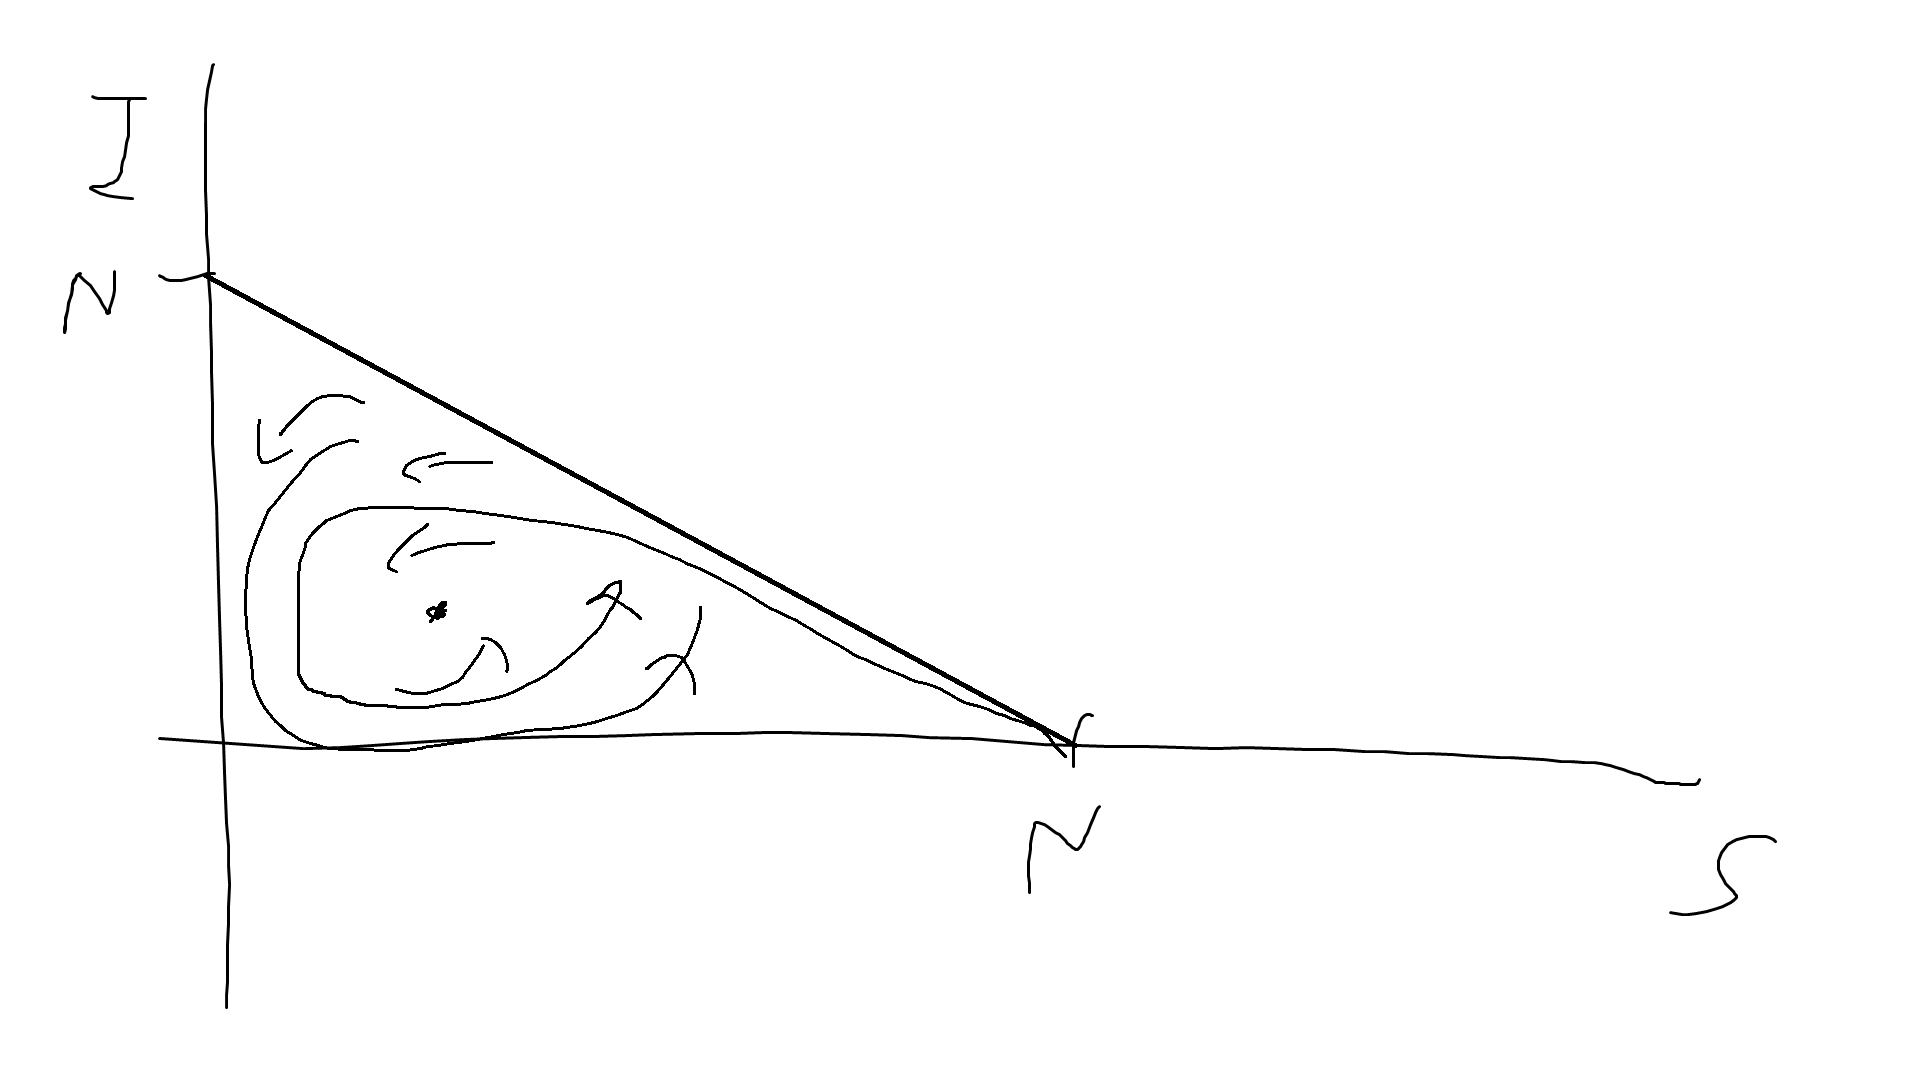
\includegraphics[scale=0.5]{image/Bio_10.png}
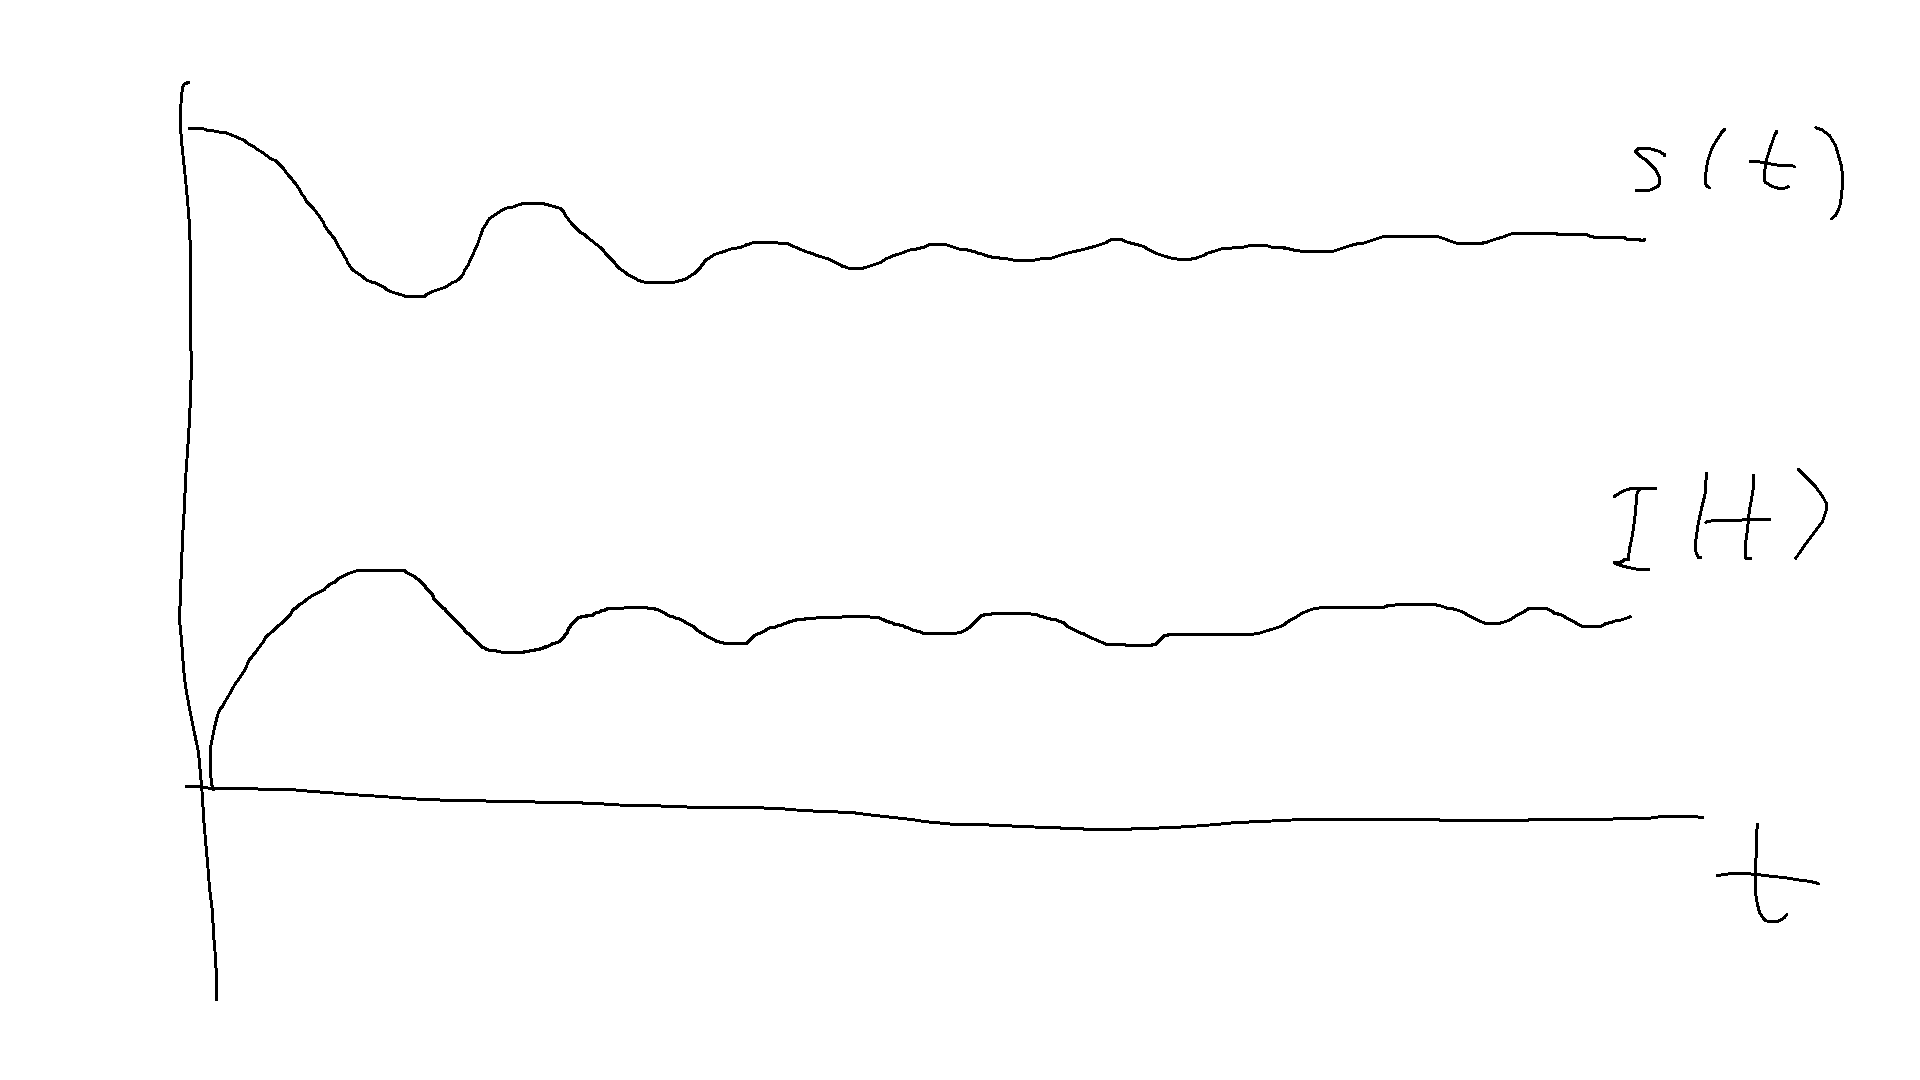
\includegraphics[scale=0.5]{image/Bio_11.png}

Time period is $T = \frac{2\pi}{\omega} = \frac{2\pi}{\sqrt{\mu\nu(R_0-1)}}$

If $\mu \gg \nu$, for example, for Measles we have $\mu \sim \frac{1}{70}$ years, $\nu \sim \frac{1}{10}$ days, $\mathcal{R}_0 \sim 20$, so the period of oscillation $T \approx 2.18$ years. Then we have the following pattern.

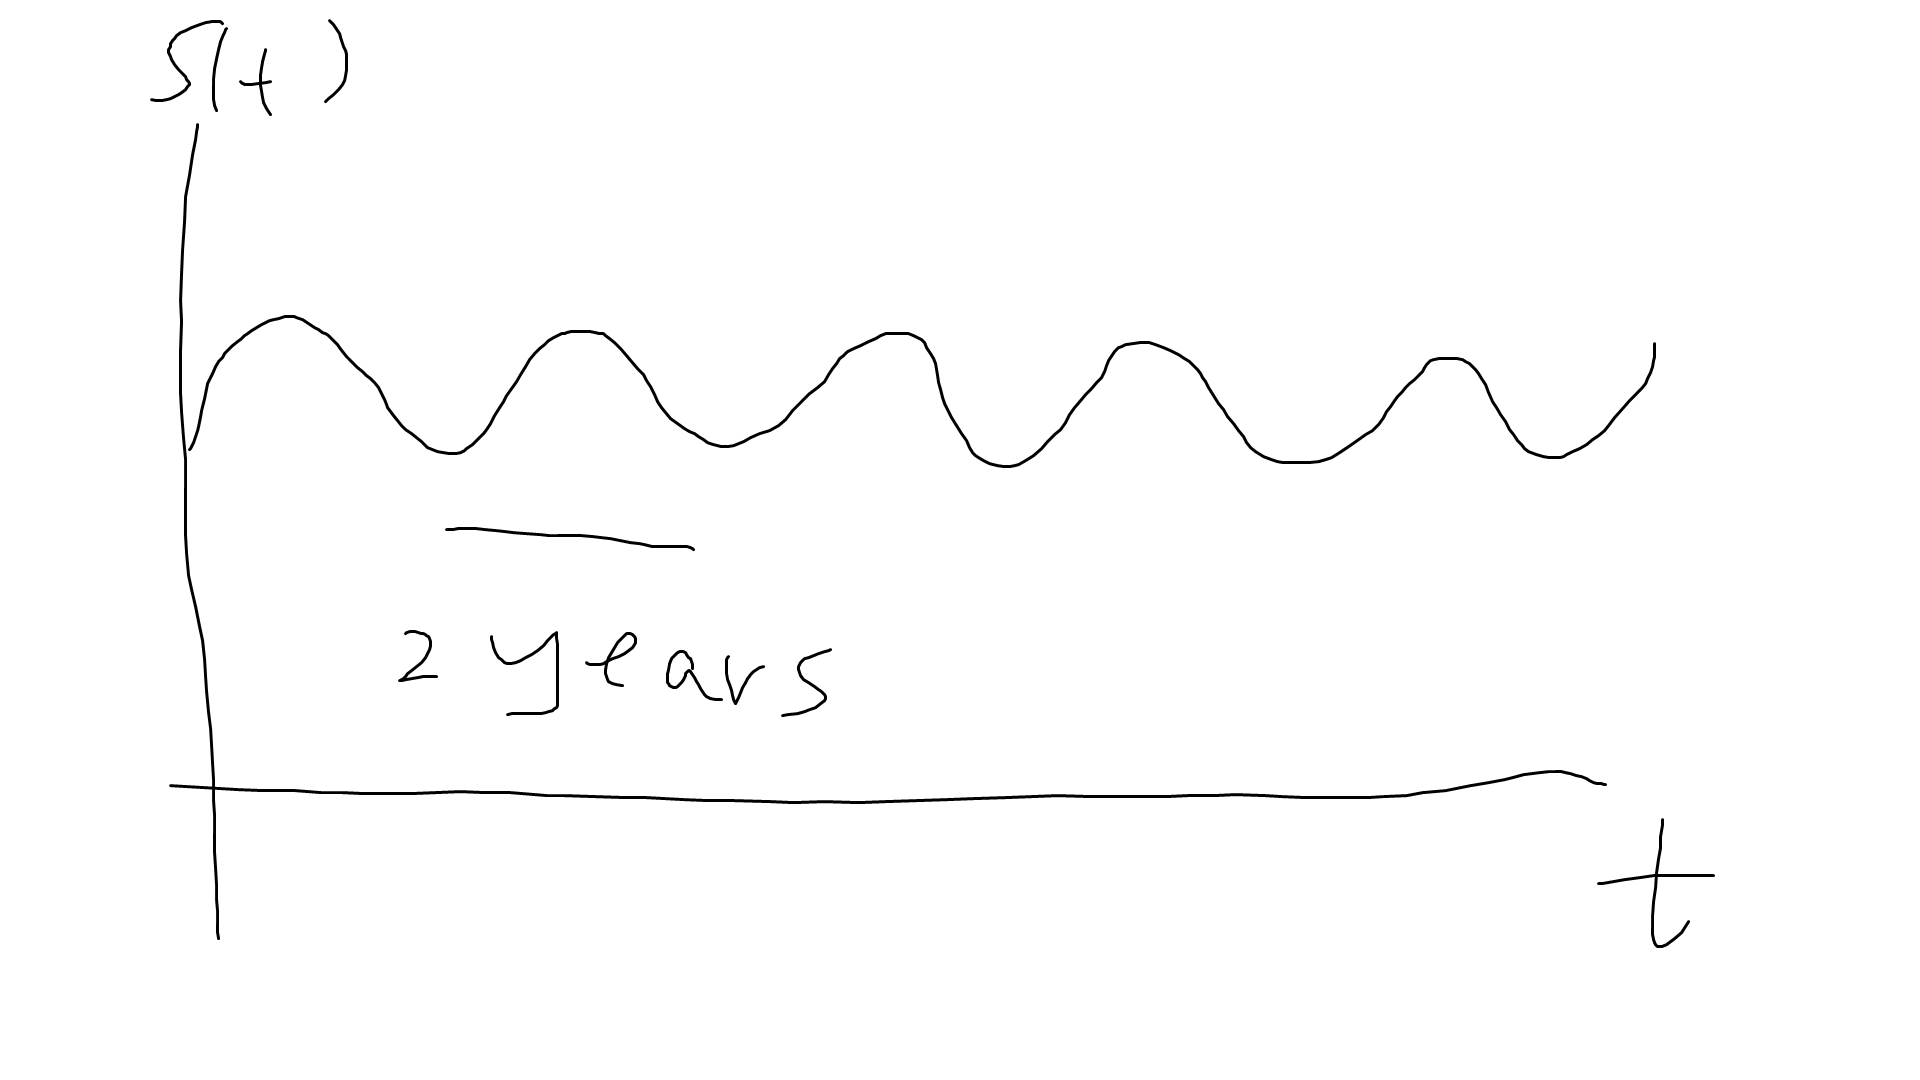
\includegraphics[scale=0.5]{image/Bio_12.png}

\newpage

\section{Enzyme Kinetics}

Enzyme is biological catalyst, which speeds up the process of reaction (substrate turning to product) without being consumed in the process.

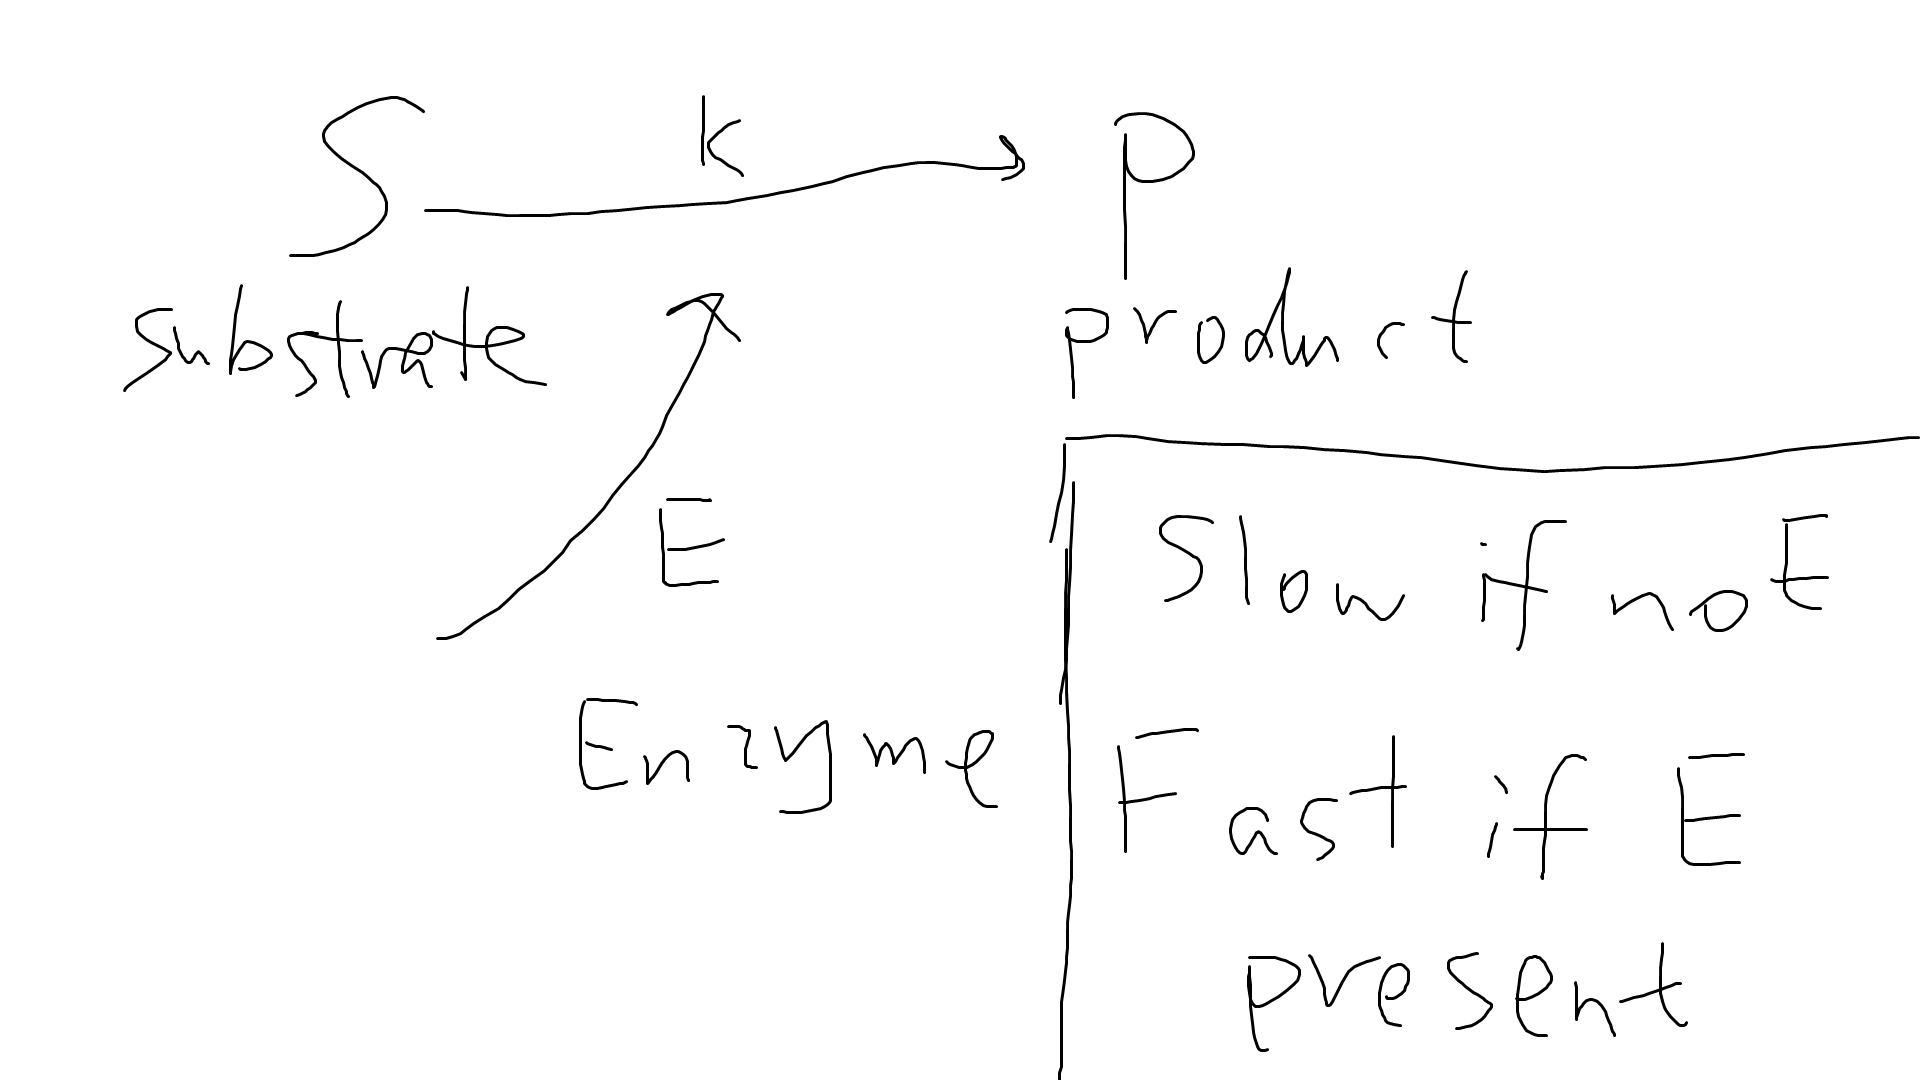
\includegraphics[scale=0.5]{image/Bio_13.png}

Suppose we have the model
\begin{equation*}
\begin{aligned}
\frac{dS}{dt} = -\bar{k}S & \text{ no enzyme}\\
\frac{dS}{dt} = -kS & \text{ enzyme present}
\end{aligned}
\end{equation*}
where $k \gg \bar{k}$.

Hypothesis: (Michaelis-Menten, $\sim$1915)
\begin{equation*}
\begin{aligned}
S + E \xrightarrow{k_1} C \text{ (complex)}\\
C \xrightarrow{k_2} S+E\\
C \xrightarrow{k_3} E+P
\end{aligned}
\end{equation*}
Under this model, we have
\begin{equation*}
\begin{aligned}
\frac{d}{dt} S &= -k_1 ES + k_2C\\
\frac{d}{dt} E &= -k_1 ES + k_2C + k_3 C\\
\frac{d}{dt} C &= k_1 ES - k_2C - k_3 C\\
\frac{d}{dt} P &= k_3 C
\end{aligned}
\end{equation*}

We see that $\frac{d}{dt} (E+C)=0$, and $\frac{d}{dt} (S+C+P)=0$. Therefore, $E+C=e_0$ is constant and $S+C+P=s_0$ is constant. There are 4 equations and 2 constraints, so we can reduce the dimension of the equation. We will choose
\begin{equation*}
\begin{aligned}
\frac{d}{dt} S = -k_1(e_0-C) S + k_2 C = -k_1e_0 S + (k_1S+k_2) C\\
\frac{d}{dt} C = k_1(e_0-C)S - k_2C - k_3C = k_1 e_0 S - (k_1S+k_2+k_3) C
\end{aligned}
\end{equation*}
We use our old trick (?) of rescaling variables by $n_S = \frac{S}{s_0}$, $n_C = \frac{C}{e_0}$, then $n_S=1$ and $n_C=0$ at $t=0$. The equations become 
\begin{equation*}
\begin{aligned}
\frac{d}{dt} n_S = -n_S + (n_S + \mu-\lambda) n_C\\
\varepsilon \frac{d}{dt} n_C = n_S - (n_S+\mu) n_C
\end{aligned}
\end{equation*}
where $\mu = \frac{k_3}{k_1s_0}, \lambda = \frac{k_2+k_3}{k_1s_0}, \varepsilon = \frac{e_0}{s_0} \ll 1$.

Steady state value of $n_C$ assuming $n_S$ is fixed:\\
$n_C = \frac{n_S}{n_S+\mu}$ as $t \to \infty$. Plug them back into $n_S$ equation, get
\begin{equation*}
\begin{aligned}
\frac{d}{dt} n_S = -n_S + (n_S+\mu-\lambda) \frac{n_S}{n_S+\mu}\\
\frac{d}{dt} n_S = -\frac{\lambda n_S}{n_S + \mu} \ (*)
\end{aligned}
\end{equation*}
This is called the Michaelis-Menten equation.

\section{Prey-predator system}
Suppose we have rabbits with number $n_R$, and foxes with number $n_F$. Our biological datum is that if there is no predation then rabbits grow unboundedly, and foxes die (as they have nothing to eat). With predation, rabbits die at a rate $b$ per capita, and foxes reproduce at a rate $c$ per capita. We have
\begin{equation*}
\begin{aligned}
\frac{d}{dt} n_R = a \cdot n_R - b n_R n_F\\
\frac{d}{dt} n_F = c n_R n_F - dn_F
\end{aligned}
\end{equation*}
we write as
\begin{equation*}
\begin{aligned}
\frac{d}{dt} n_R = n_R (1-n_F)\\
\frac{d}{dt} n_F = -\alpha n_F (1-n_R)
\end{aligned}
\end{equation*}
This has fixed points $(0,0)$ and $(1,1)$, and has Jacobian
\begin{equation*}
\begin{aligned}
\begin{pmatrix}
1-n_F & -n_R\\
\alpha n_F & -\alpha(1-n_R)
\end{pmatrix}
\end{aligned}
\end{equation*}
evaluate at the two fixed points, we see that $(0,0)$ is unstable (actually a saddle), and the $(1,1)$ fixed point has eigenvalue (of Jacobian) $\pm i\sqrt{\alpha}$. Since the real part is 0 we don't know (yet) whether it is stable or not. We have to solve the equations of motion:
\begin{equation*}
\begin{aligned}
d n_R = n_R (1-n_F) dt\\
d n_F = -\alpha n_F (1-n_R) dt
\end{aligned}
\end{equation*}
so $\frac{d n_R}{dn_F} = \frac{n_R (1-n_F)}{-\alpha n_F(1-n_R)}$, i.e. $\alpha \frac{1-n_R}{n_R} dn_R = -\frac{1-n_F}{n_F} dn_F$ so $\alpha(\log n_R - n_R) = -(\log n_F - n_F) + c$. We get $H(n_R,n_F) = \alpha(n_R - n_R) + \log n_F - n_F = $constant, where $H(n_R,n_F)$ is the integral of motion. So we should observe the number $n_R$ and $n_F$ show a pattern of oscillation with some period $T$ which we wish to find.

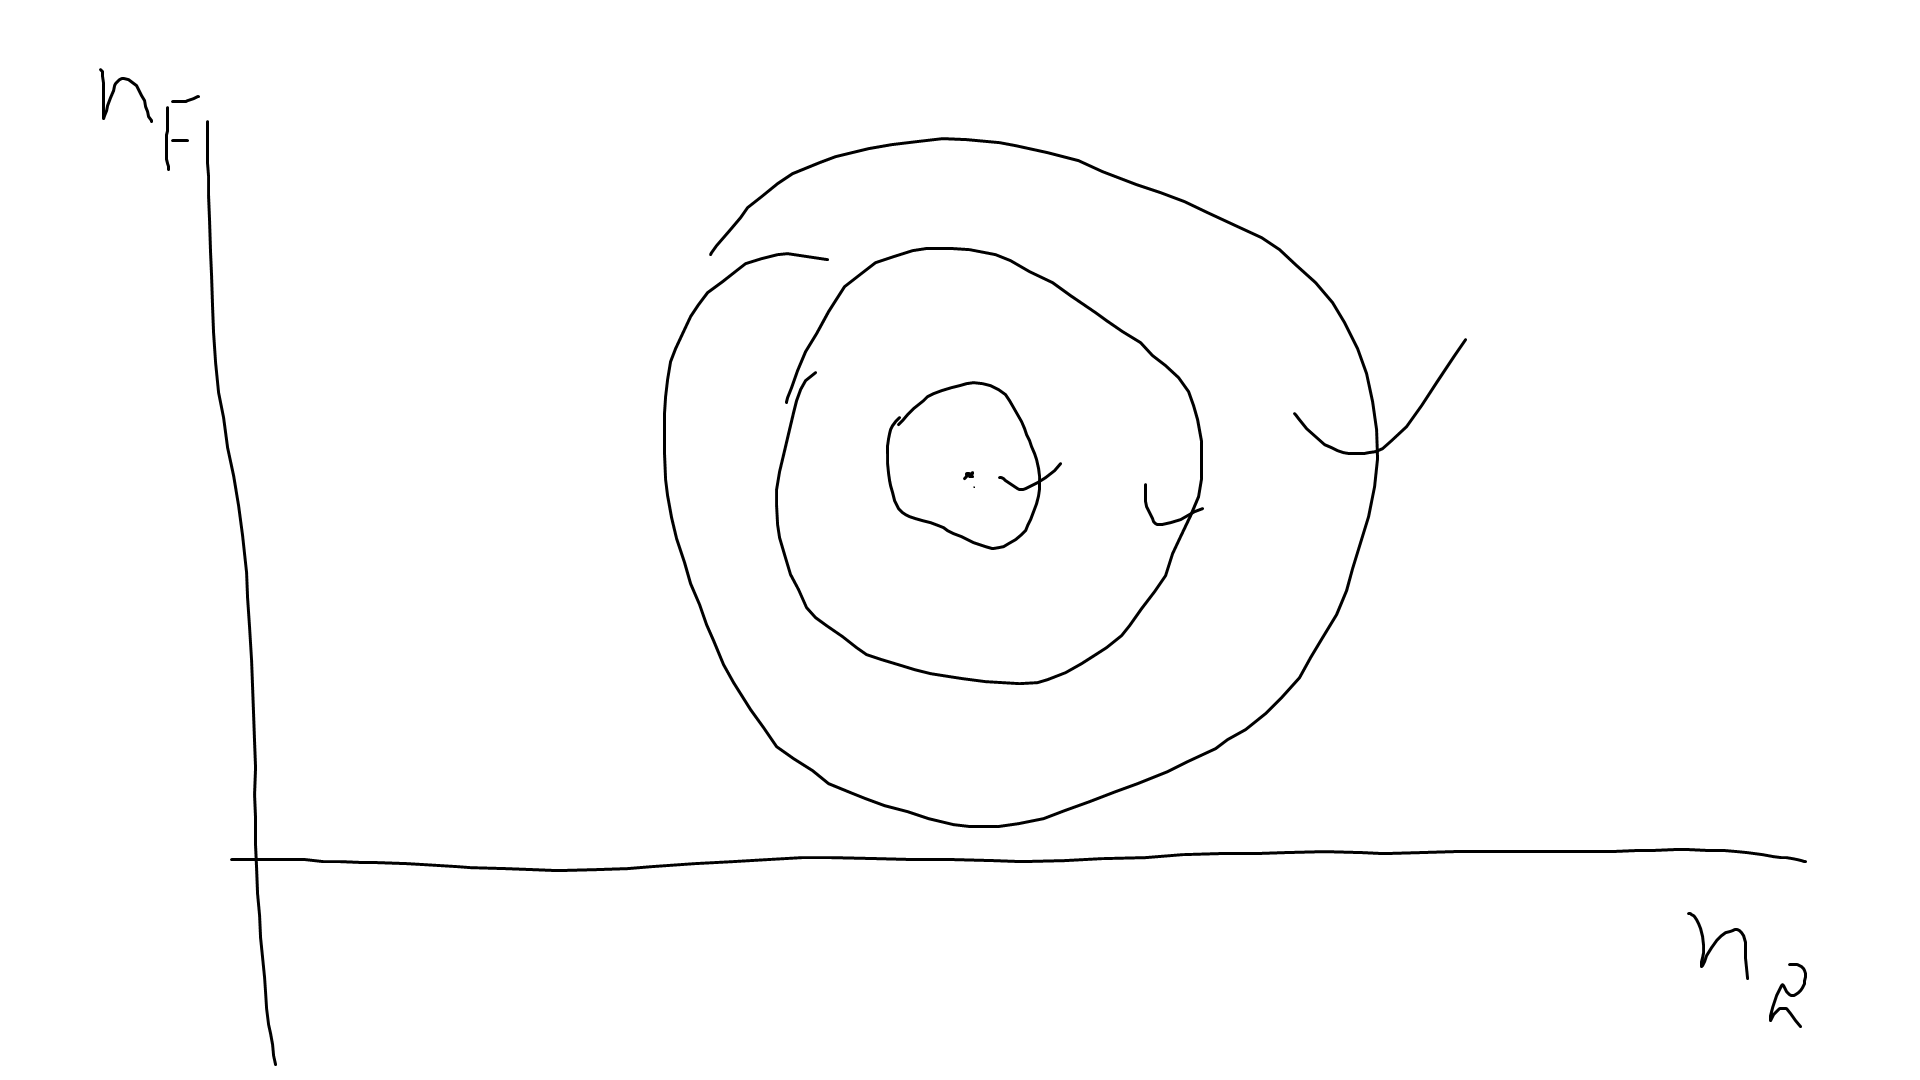
\includegraphics[scale=0.5]{image/Bio_14.png}

We'll get $T=1$ after some interesting contour integration (no idea) $\oint d(\ln n_R ) = \int_0^\pi (1-n_F)dt$.

What if both are hunted upon (say by a disease)? Let the death rate of rabbits and foxes be $\lambda_R$ and $\lambda_F$ respectively. Then $\frac{d}{dt} n_R = an_R - bn_Rn_F - \lambda_R n_R$, $\frac{d}{dt} n_F = cn_Rn_F - dn_R-\lambda_F n_F$. We introduce a shift parameter $a \to a-\lambda_R$, $d \to d+\lambda_F$, then we find that there is a shift on the fixed points: the fixed point in original variables is $(n^*_R,n^*_F) = (d/c,a/b)$. Now the new fixed point becomes $(n^*_R$, $n^*_F) =((d+\lambda_F)/c,(a-\lambda_R)/b)$.

Fragility of ecosystems: if we add competition:

\begin{equation*}
\begin{aligned}
\frac{d}{dt} n_R &= n_R(1-n_F) - \varepsilon_R n_R^2\\
\frac{d}{dt} n_F &= -\alpha n_F(1-n_R) - \alpha \varepsilon_F n_F^2
\end{aligned}
\end{equation*}
After doing the same calculation we get
\begin{equation*}
\begin{aligned}
n_R^* &= \frac{1+\varepsilon_F}{1+\varepsilon_R\varepsilon_F}\\
n_F^* &= \frac{1-\varepsilon_F}{1+\varepsilon_R\varepsilon_F}\\
J^* &= \begin{pmatrix}
-\varepsilon_R n_R^* & -n_R^*\\
\alpha n_F^* & -\alpha\varepsilon_F n_F^*
\end{pmatrix}
\end{aligned}
\end{equation*}
and only the (2,1) entry is positive, so $\tr J <0$, $\det J >0$. So this fixed point now becomes stable.

Let's consider another model, the Fitzhugh-Nagumo model:
\begin{equation*}
\begin{aligned}
\frac{d}{dt} n_1 = c(n_2+n_1 - \frac{1}{3} n_1^3 + \mathcal{L}(t))\\
\frac{d}{dt} n_2 = -\frac{1}{c} (n_1 - a+bn_2)
\end{aligned}
\end{equation*}
where $\mathcal{L}(t)$ is an external signal, which can depend on time.

Nullclines(maybe something in dynamical systems?):\\
\begin{equation*}
\begin{aligned}
\frac{d}{dt} n_1 = 0 \implies n_2 = -n_1 + \frac{1}{3} n_1^3\\
\frac{d}{dt} n_2 = 0 \implies n_2 = \frac{a-n_1}{b}
\end{aligned}
\end{equation*}
where $\mathcal{L}(t) = 0$. The parameter bounds are $0<b\leq 1, 1-\frac{2}{3} b < a < 1, c \gg 1$. If we plot the two graphs we get fixed point at $n_1>0,n_2<0$, a stable focus.

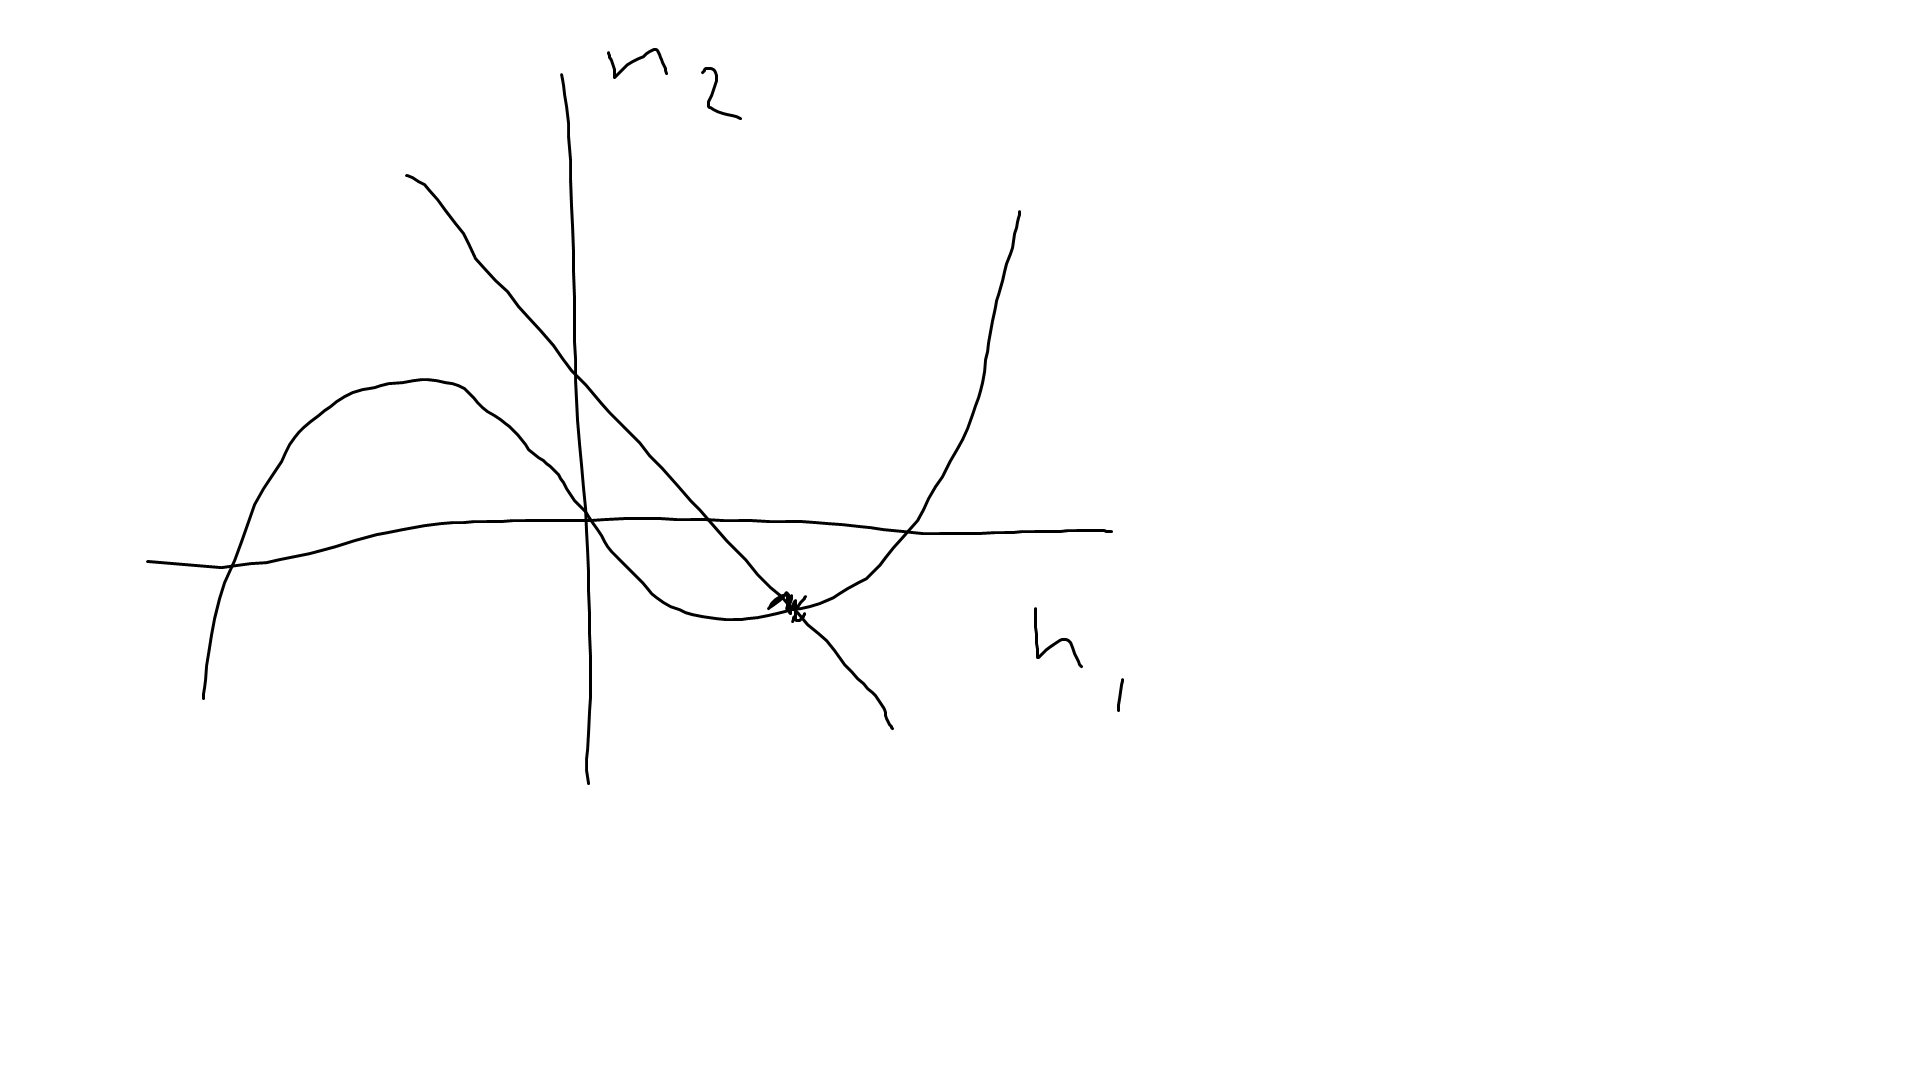
\includegraphics[scale=0.5]{image/Bio_15.png}

If we now add $\mathcal{L}(t)$, we are essentially moveing the cubic curve upwards. There are three cases in terms of the magnitude added:\\
(1) small: nothing interesting happens, the fixed point just moves by a bit;\\
(2) medium: $n_2$ spikes up first, then falls back to the fixed points;
(3) large: fixed points lose stability; $n_2$ oscillate like the above diagram, with spikes after certain periods.

\iffalse

\begin{equation*}
\begin{aligned}

\end{aligned}
\end{equation*}
\fi


\end{document}
